\section{Systematic Uncertainties}
\label{sec:analysis:systematics}


Various sources of systematic uncertainties are described in this sections. As discussed in Section~\ref{sec:analysis:method}, the treatment of systematics differs between the two analysis approaches: the shape analysis makes use of nuisance parameters; the counting analysis is carried out varying each systematic individually and assessing the variation on the estimates of the branching fractions. This section first presents the sources of systematic uncertainties and then estimates their impacts to the measurement in shape and counting analysis.


\subsection{Sources of Systematic Uncertainties}
\label{sec:analysis:systematics:source}


\subsubsection{Luminosity} 
The uncertainty on the CMS luminosity measurement is taken to be 2.5\% for the 2016 run~\cite{CMS-PAS-LUM-17-001}.  This uncertainty effects the overall scale of all predicted yields in a fully correlated manner. 
% In shape analysis, it is handled as a normalization nuisance parameter. In counting analysis, its effect on signal simulations is cancelled and effect on background simulation gets propagated.


\subsubsection{Data-driven estimations for QCD background}

The uncertainty is split into four normalization parameters: one for each of the final states \cet, \cmt, \ceh, and \cmh.  

\subsubsection{Cross section for simulated processes} 

We assign the following uncertainties to the cross sections for simulated processes.

\begin{itemize}
    \item \ttbar: 5\%, (and PDF, $\alpha_{s}$, $\mu_{R}/\mu_{F}$ in shape analysis)
    \item \tW:    5\%
    \item \zjets: 10\%, (and PDF, $\alpha_{s}$, $\mu_{R}/\mu_{F}$ in shape analysis)
    \item \wjets: 10\%
    \item \gjets: 10\%
    \item diboson: 10\%
\end{itemize}
% For diboson, shape analysis treats \PWW as a signal and its cross-section is not constrained.
Since shape analysis also incorporates \zjets control regions and is sensitive to the \ttbar cross-section, the cross-section of \zjets and \ttbar is further decomposed into extra nuisance parameters, including PDF, $\alpha_{s}$, $\mu_{R}/\mu_{F}$. The counting analysis does not have \zjets control regions and is insensitive to \ttbar cross-section due to the construction of ratio of channels. So overall uncertainties of \ttbar and \zjets are used.

\subsubsection{\WW \pt reweighting}
The shape analysis treats \WW as a signal. The reweighting of the \WW \pt is accounted for by including two nuisance parameter for the resummation and factorization variations as described in section~\ref{sec:analysis:calibration:genlevel}. In the \ttbar signal region employed by the counting analysis, there is little contamination from \WW process. Thus the \WW \pt reweighting and associated systematic effects are neglected.

\subsubsection{top \pt reweighting}
Top \pt reweighting is applied in nominal case because it is observed as unnecessary, but is used to estimate the associated uncertainties. In shape analysis, the uncertainty on the top \pt scale is included as a one-sided morphing templates generated based on previous top studies in shape analysis and it turns out to be highly constrained. In counting analysis, the construction of ratios allow cancellations of \ttbar related systematics and 1\% of the top \pt scale is used as the size of uncertainty, which gets propagated through the parameter extraction.


\subsubsection{Pileup}

Each event is weighted with a scale factor to account for differences in the pileup spectrum between data and simulation.  The uncertainty on the event weights is mainly due to the uncertainty on the minimum bias cross section.  The nominal minimum bias cross section is $69.2 \pm 3.18~\text{mb}$. The effect of the uncertainty is propagated through the analysis by calculating the distribution of pileup in data while varying the cross section up and down by one standard deviation.  

\subsubsection{Trigger efficiency}

% The uncertainty due to the trigger efficiency scale factors is accounted for by saving the uncertainty of each weight and including the uncertainty in the bin uncertainty of the template histograms.  

\begin{itemize}
    \item \textit{single muon}: 0.5\% normalization uncertainty on all categories where the triggering lepton is a muon.
    \item \textit{single electron}: a $\pt$ and $\eta$ dependent correction is applied to events triggerred with single electron trigger. The correction and uncertainty is measured with tag-and-prob approach described in \ref{sec:analysis:calibration:trigger}. The uncertainty accounts for the statistical uncertainty, the variation due the triggering of the tag lepton, and variation due to the probe electron.
\end{itemize}

\subsubsection{Muon reconstruction}
    \begin{itemize}
    \item \textit{identification/isolation}: the uncertainties are accounted for each muon and are based on values provided by the POG. 
    \item \textit{energy scale}: to account for the muon energy scale, the muon \pt is varied by $\pm 1 \sigma$ (0.2\%).
    \end{itemize}

\subsubsection{Electron reconstruction}
    \begin{itemize}
        \item \textit{identification/isolation}: the uncertainties provided per electron are taken from values provided by the POG.
        \item \textit{reconstructions}: treated the same as the identification uncertainty.  Scale factors and their uncertainties are only $\eta$ dependent. 
        \item \textit{energy scale}: The electron energy scale is assumed to be know at the 0.5\% level, and is assigned a  nuisance parameter that modifies the change to the shape of the relevant kinematic quantity.
        %\item \textit{resolution}
    \end{itemize}

\subsubsection{Tau reconstruction}
    \begin{itemize}
        \item \textit{identification}: the $\PGth$ POG recommends a 5\% uncertainty on the scale factor applied to simulation. In shape analysis, because a control region is included to provide an \emph{in situ} evaluation of the $\PGth$ efficiency scale factor, the scale factors are included as \pt-dependent nuisance parameter in seven \pt bins.
        
        \item \textit{$jet\rightarrow\PGth$}: scale factors and uncertainties for jets faking taus were derived based on a dilepton plus reconstructed tau control region.  A nuisance parameter is assigned to each \pt bin used to measure the scale factor and an overall normalization nuisance parameter is assigned to account for any difference in rate between light and heavy jets.
        
        \item \textit{$\Pe\rightarrow\PGth$}: a single normalization nuisance parameter is included to templates where an electron is misreconstructed as a hadronically decaying tau. The counting analysis neglects this uncertainty because the contribution of electron faking \PGth is only sizable in $\PZ \to \PGte \PGth$ control region, not considered by the counting analysis.  
        
        \item \textit{energy scale}: the tau energy scale is corrected in correspondence with POG recommendations and an uncertainty of 1.2\% per decy mode is assigned.  These are included as three shape uncertainties depending on the reconstructed decay mode of the hadronically decaying tau. 
    \end{itemize}

    In addition, the uncertainties of different \PGth decay widths are investigated. Currently the world average of the major \PGth decay widths have about 0.5-1.0\% uncertainties. Five highest \PGth branching fractions include 
    \begin{equation*}
    \begin{split}
    &   \mathcal{B}(\PGth\to \PGp^\pm)        = 0.1082(5), \quad 
        \mathcal{B}(\PGth\to \PGp^\pm \PGp^0)  = 0.2549(9), \quad 
        \mathcal{B}(\PGth\to \PGp^\pm2\PGp^0)  = 0.0926(10),\\
    &   \mathcal{B}(\PGth\to3\PGp^\pm)        = 0.0931(5), \quad
        \mathcal{B}(\PGth\to3\PGp^\pm \PGp^0)  = 0.0462(5).           
    \end{split}
    \end{equation*}
    \noindent Since different decay modes are reconstructed separately by the CMS \PGth identification and thus have different efficiencies. The uncertainties of different \PGth widths could propagate to the \PGth identification efficiencies and lead to some impacts on the final results. To decide the impact, we tag the generator-level decay mode of reconstructed \PGth and vary the event weight accounting to the relative uncertainty of the tau decay branching fraction. Figure~\ref{fig:analysis:systematics:tauhDecayMode} shows the distribution of gen-level \PGth decay modes of $\ttbar \to \cmt$ simulated events selected in the \cmt channel. Considering the above five major \PGth decay mode, the corresponding uncertainties on the \BWl are found to be less then 0.1\% relatively, small enough to neglect.
    
    \begin{figure}
    \centering
    \includegraphics[width=0.99\textwidth]{chapters/Analysis/sectionSystematics/figures/tauBr/tauhDecay_mutau.png}
    \caption{Distribution of gen-level \PGth decay modes of $\ttbar \to \cmt$ simulated events selected in the \cmt channel.}
    \label{fig:analysis:systematics:tauhDecayMode}
\end{figure}




\subsubsection{Jet reconstruction}

    Jet systematics impact the analysis by modifying the acceptance of
    events in the various jet multiplicity categories.  With that in
    mind, the uncertainty is taken into account by varying the various
    sources of jet uncertainties and assessing the resulting effect on
    the jet and \PQb tag multiplicities.

    \begin{itemize}
        \item \textit{energy scale}: the jet energy scale is varied by
            the various uncertainty sources on the jet energy
            corrections provided by the JetMET POG.  These are included
            as 18 shape nuisance parameters (the lepton kinematic quantities
            which are fit are generally not affected by variation of the
            jet energy scale, but migration between different \PQb tag
            categories does happen)
        \item \textit{resolution}: the jet energy is corrected in
            simulation to account for the difference in resolution
            between data and simulation.  The correction is applied per
            jet and is dependent on the jet \pt.  Consequently, there is
            an associated uncertainty.  The overall effect of this is
            estimated by varying the scale factor up and down one
            standard deviation and propagating the effect to the
            morphing templates.
    \end{itemize}

\subsubsection{b-tagging}
    
The \PQb tag modelling in simulation is corrected to better describe the
data based on scale factors.  The uncertainty on the correction is
assessed based on up and down variations of \PQb tagging and mistagging
scale factors supplied by the \PQb tag POG.  The \PQb tag uncertainties are
factorized based on the various sources of uncertainty considered in the
calculation of the scale factors.  The variation is propagated through
the analysis through the inclusion of shape nuisance parameters for both
b tagging and mistagging variation.




\subsubsection{Theory/simulation modelling}

In addition to the normalization uncertainties coming from PDF, QCD
scale, and uncertainty on $\alpha_{s}$, several other theory
uncertainties are accounted for.  These are only included for $\ttbar$
processes and are applied as recommended by TOP PAG.

\begin{itemize}
    \item \textit{ISR/FSR}: variations to $\alpha_{S}$ affecting both
        ISR and FSR are evaluated based on dedicated \ttbar MC samples.
        This is done for ISR and FSR independently.  These variations are
        propagated through the analysis through morphing templates.
    \item \textit{ME-PS matching scale}: matrix element to parton shower
        matching is regulated at the generator level by the \textit{hdamp}
        parameter.  This parameter is varied from the nominal value of
        $1.58^{+0.66}_{-0.59}$ in dedicated MC samples and propagated 
        through morphing templates.
    \item \textit{Underlying event}: modelling of the underlying event
        is dependent on the Pythia tune that is used (in the case of this
        analysis, CUETP8M2T4)~\cite{CMS-PAS-TOP-16-021}.  Dedicated samples
        are generated varying the appropriate parameters and the variation
        in efficiency is propagated through the analysis with morphing
        templates.
        %(\emph{Not included in this iteration})
\end{itemize}

There are two issues with these uncertainty sources that are worth
considering.  The first is that the variations due to these sources of
uncertainty are estimated from dedicated MC samples.  This leads to a
fairly sizeable statistical uncertainty, and can lead to exagerated
uncertainties and strange behavior in the morphing templates (e.g., both
the up and down variation will predict yields below/above the nominal
sample).  Also, the size of the uncertainty resulting from the FSR
variation is very large (up to 20\%) in the \ceh categories.  This
level of variation would be corrected for in the scale factors
accounting for the difference in ID/misID efficiency for identified
$\PGth$ candidates, and that uncertainty in general would be much
smaller, below $5\%$. 




% Four dedicated MC samples are used for the \ttbar theoretical uncertainties,
% including FSR, ISR, matrix element parton shower (MEPS), and underline events (UE).
% Based on the four dedicated and the nominal \ttbar samples,
% the shape analysis obtains four types of the template morphine,
% while the counting analysis propagates the four deviations of signal efficiency.

% However, it is noticed that variations of theoretical parameters in these
% four dedicated MC samples could have a large influence on the $\PGth$ identification efficiency
% and the $j\to \PGth$ misidentification rate. 
% Since the uncertainty of the $\PGth$ identification efficiency and the $j\to \PGth$ misidentification rate
% are accounted for separately, the changes related to the tau identification 
% in the dedicated \ttbar samples should be removed to avoid double counting.
% Thus a correction is needed for these dedicated samples.
% Such that, the tau identification and misidentification in the dedicated samples 
% are kept the same as the nominal \ttbar sample.

To derive the correction for these dedicated MC samples, we calculate the
probabilities of reconstructing taus in the nominal and dedicated \ttbar events.
The origins of the reconstructed taus are tagged based on the matching to the
gen-level particles. Both Tight and VTight WP of tau identification are
considered. The changes in the tau id and misid due to the FSR up and down 
variation are shown in Figure~\ref{fig:analysis:systematics:sf_fsr}. The changes
due to the ISR, MEPS, UE up and down variations are shown in Figure~\ref{fig:analysis:systematics:sf_isr_MEPS_UE}.
It is clear that the FSR has a considerable impact on the \PGth id and misid that 
needs removal, while the effect from the ISR, MEPS and UE are neglectable.


\begin{figure}
    \centering
    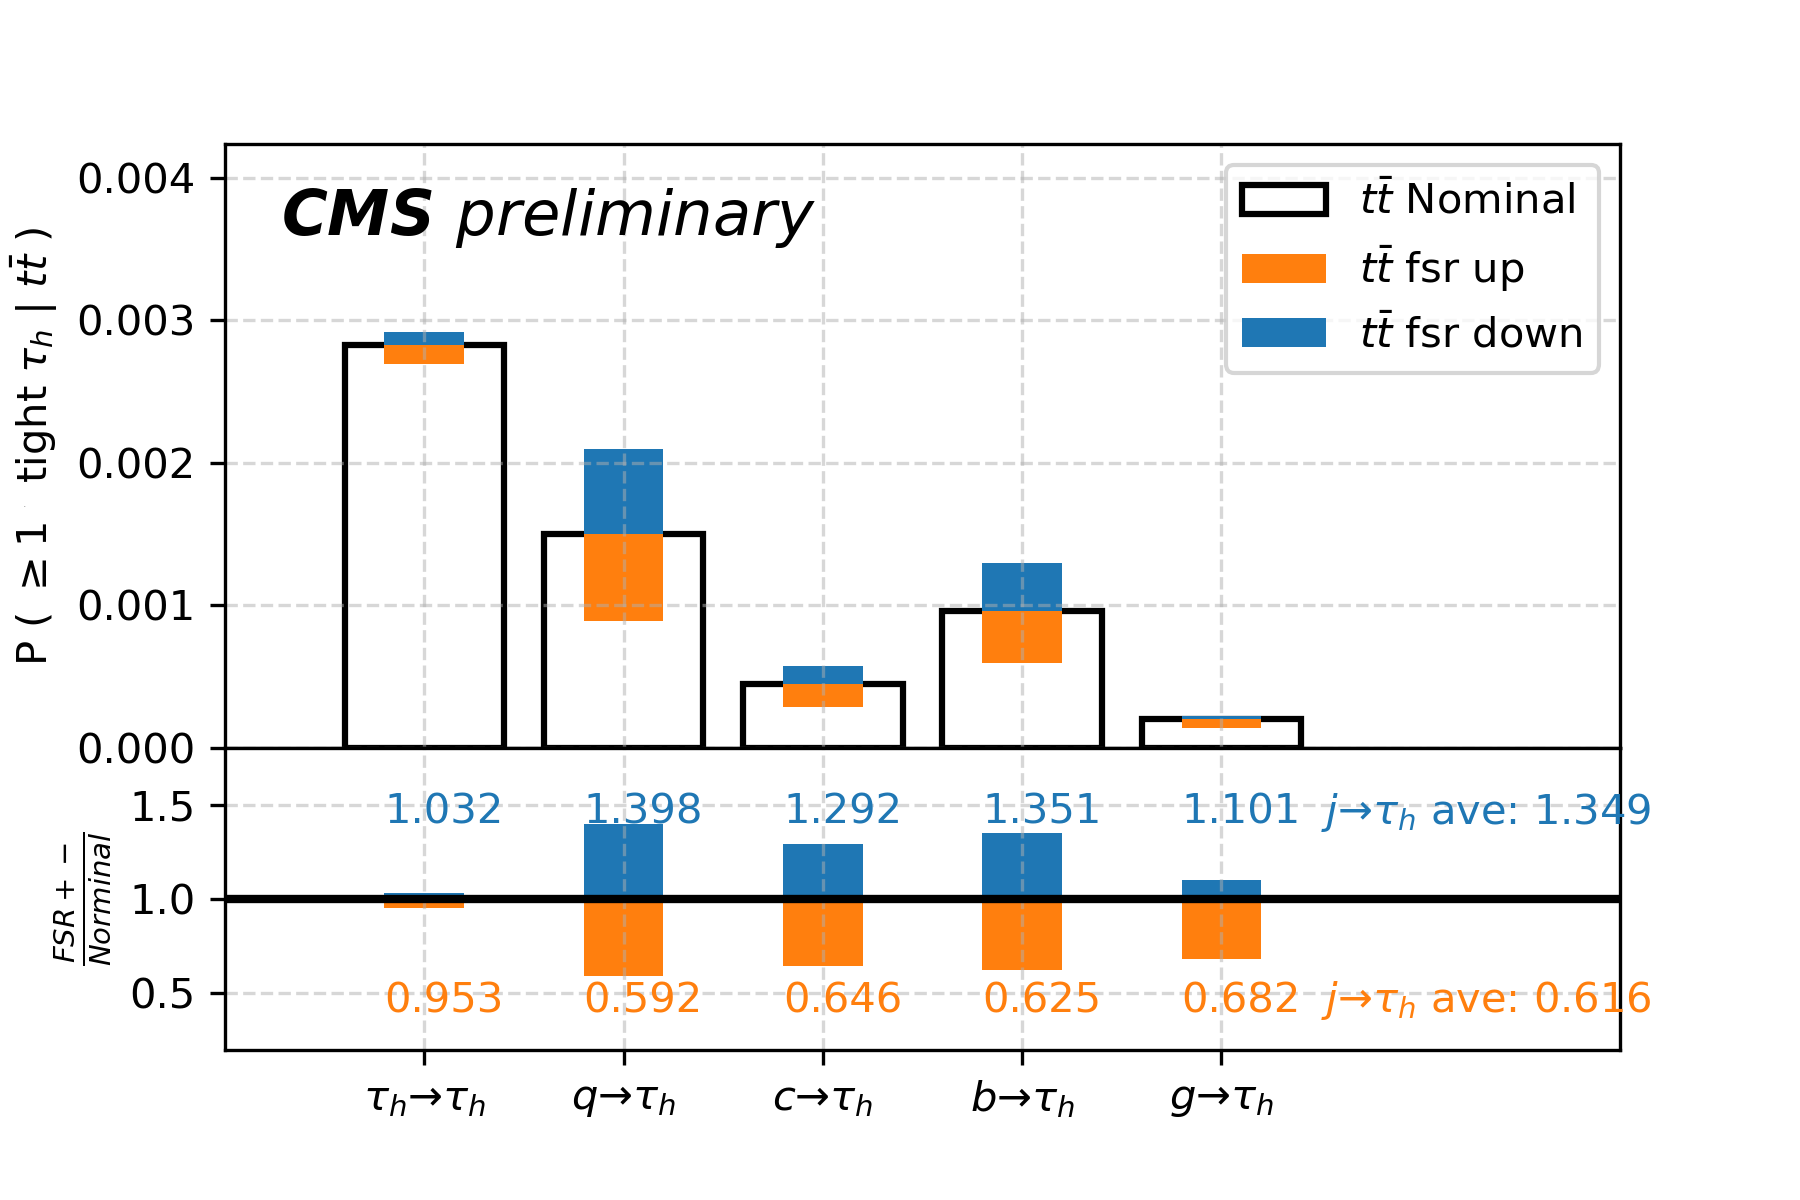
\includegraphics[width=0.49\textwidth]{chapters/Analysis/sectionSystematics/figures/ttTheoretical/2020_MCRatio_fsr_tauGenFlavor_tauTight.png}
    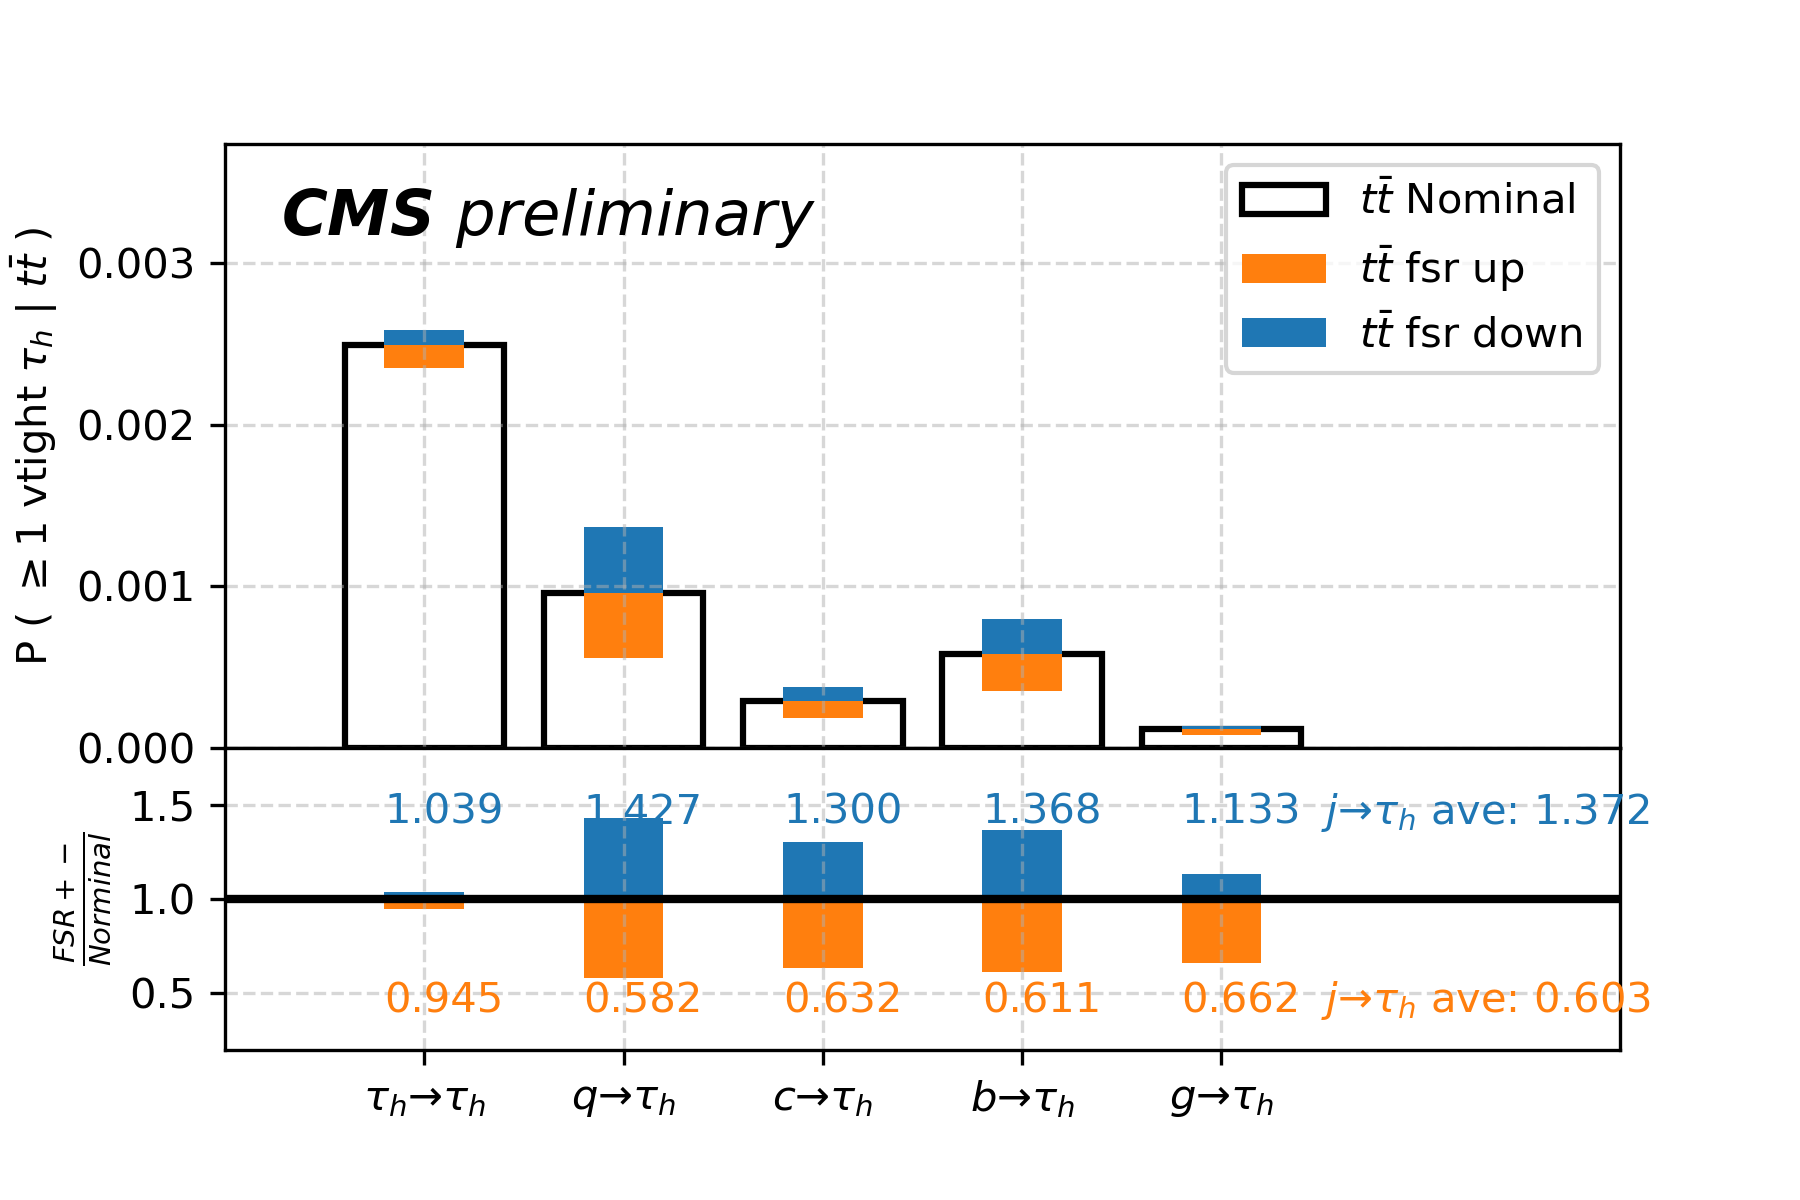
\includegraphics[width=0.49\textwidth]{chapters/Analysis/sectionSystematics/figures/ttTheoretical/2020_MCRatio_fsr_tauGenFlavor_tauVTight.png}
    \caption{Effect of final state radiation on the $\PGth$ identification and $j \to \PGth$ misidentification obtained from the dedicated and the nominal \ttbar samples. 
    The Tight and VTight WP are shown on the left and right, respectively.
    }
    \label{fig:analysis:systematics:sf_fsr}
\end{figure}

\begin{figure}
    \centering
    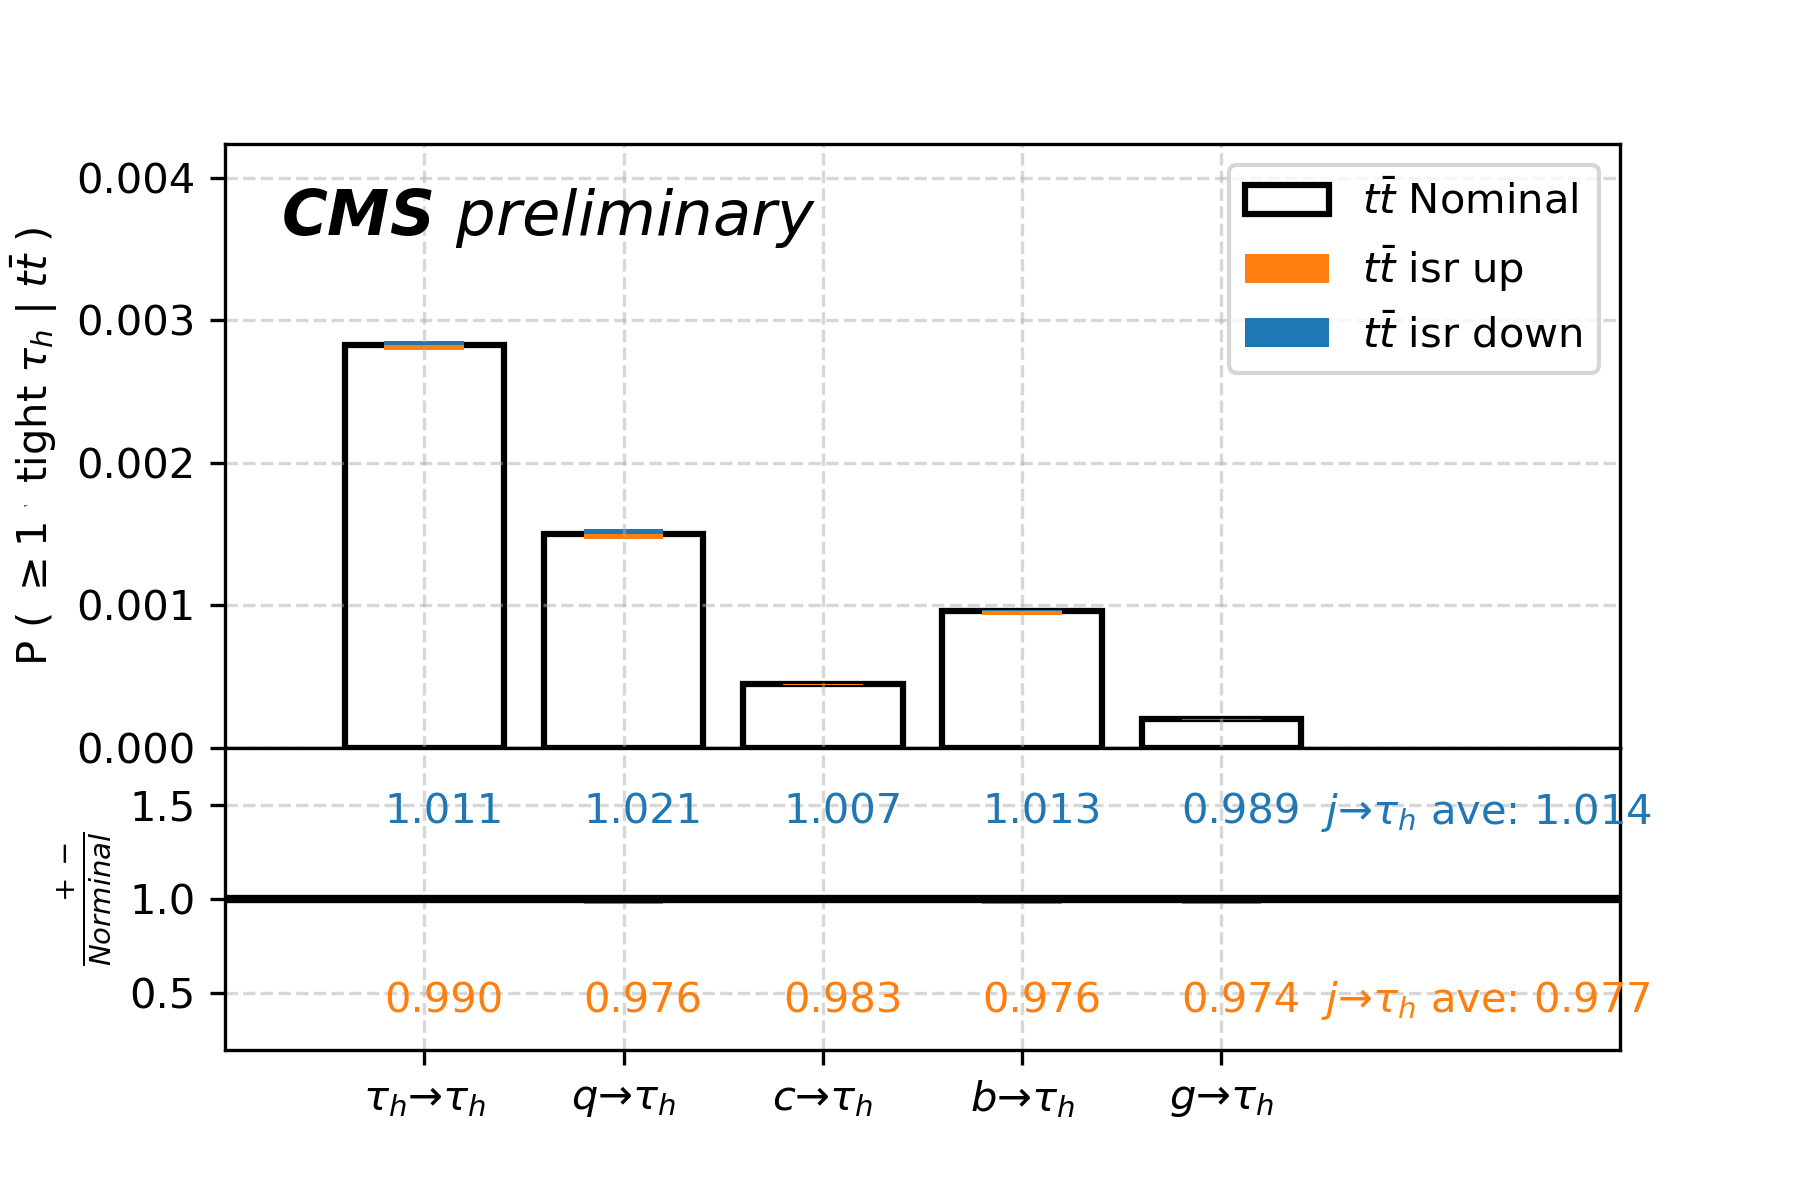
\includegraphics[width=0.49\textwidth]{chapters/Analysis/sectionSystematics/figures/ttTheoretical/2020_MCRatio_isr_tauGenFlavor_tauTight.png}
    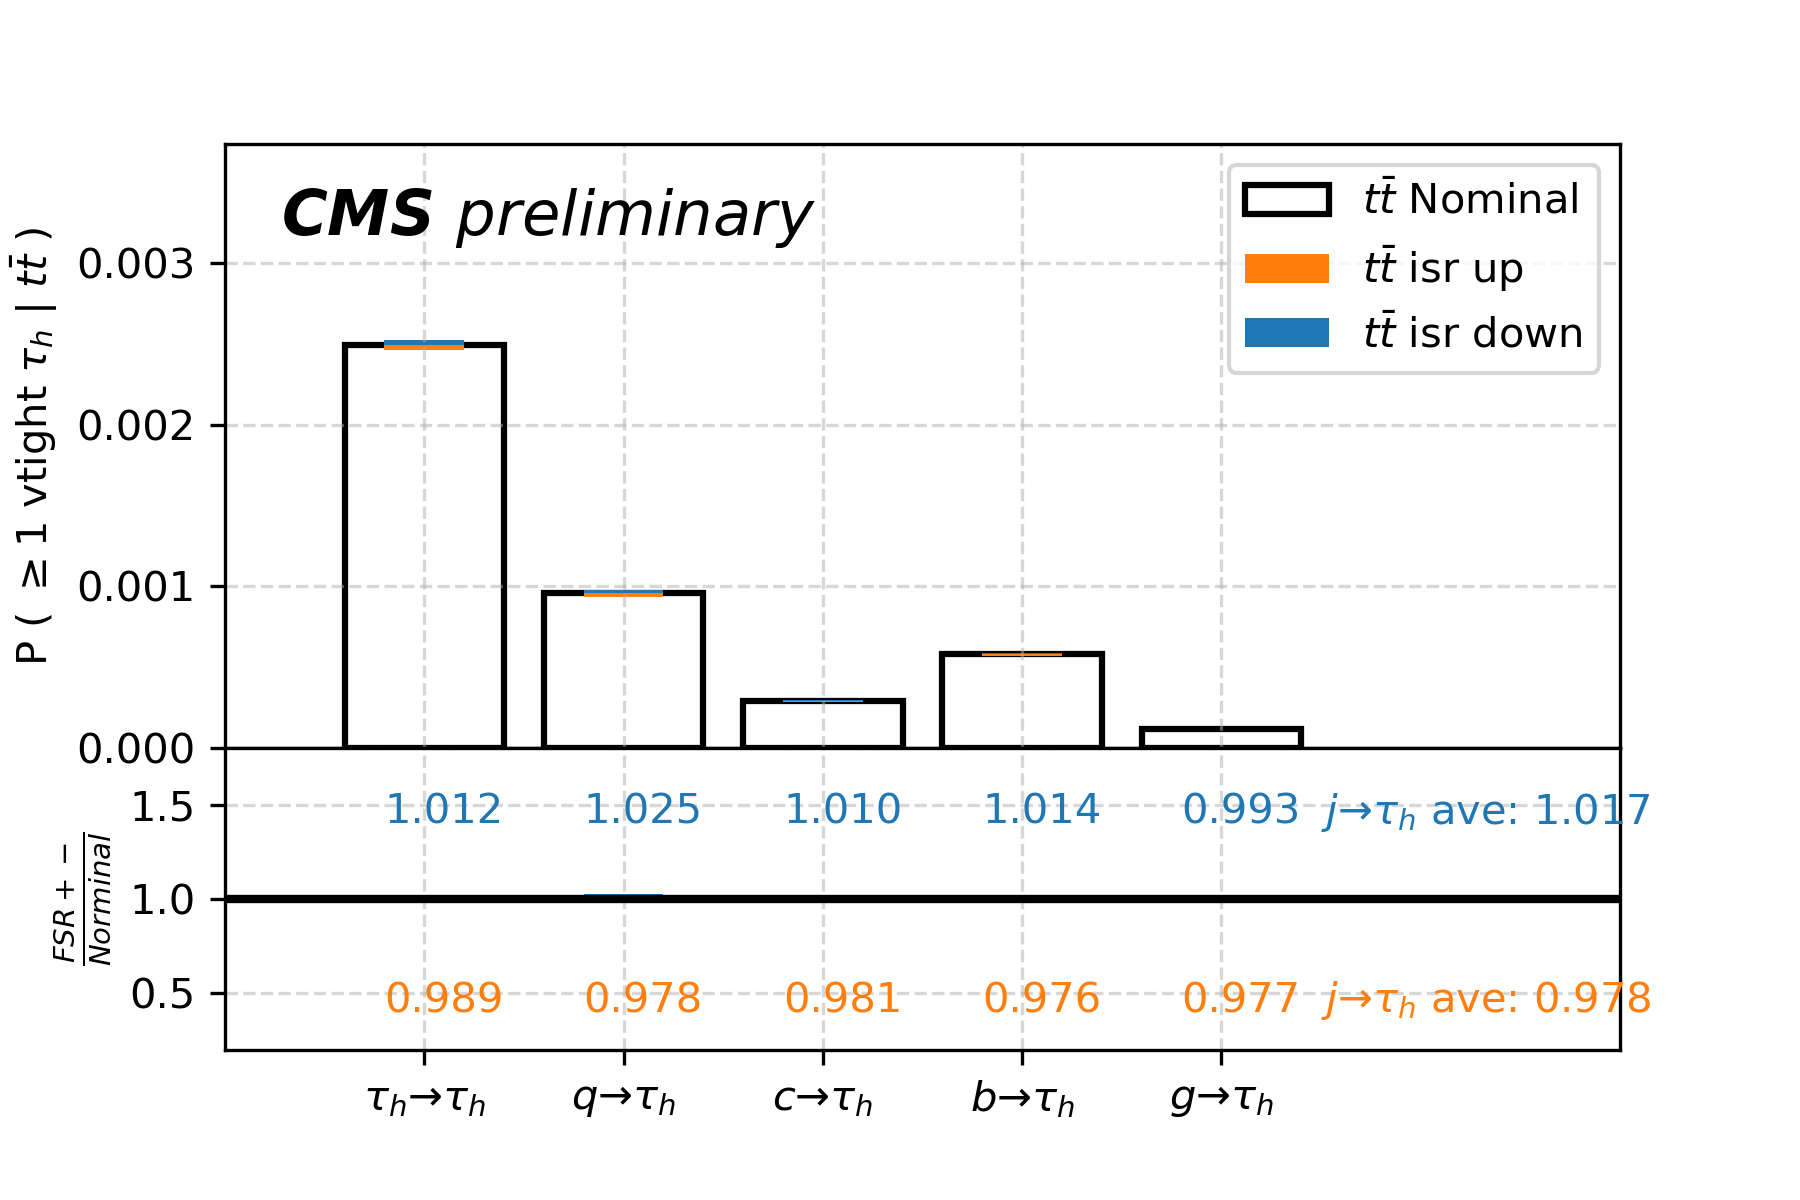
\includegraphics[width=0.49\textwidth]{chapters/Analysis/sectionSystematics/figures/ttTheoretical/2020_MCRatio_isr_tauGenFlavor_tauVTight.png}
    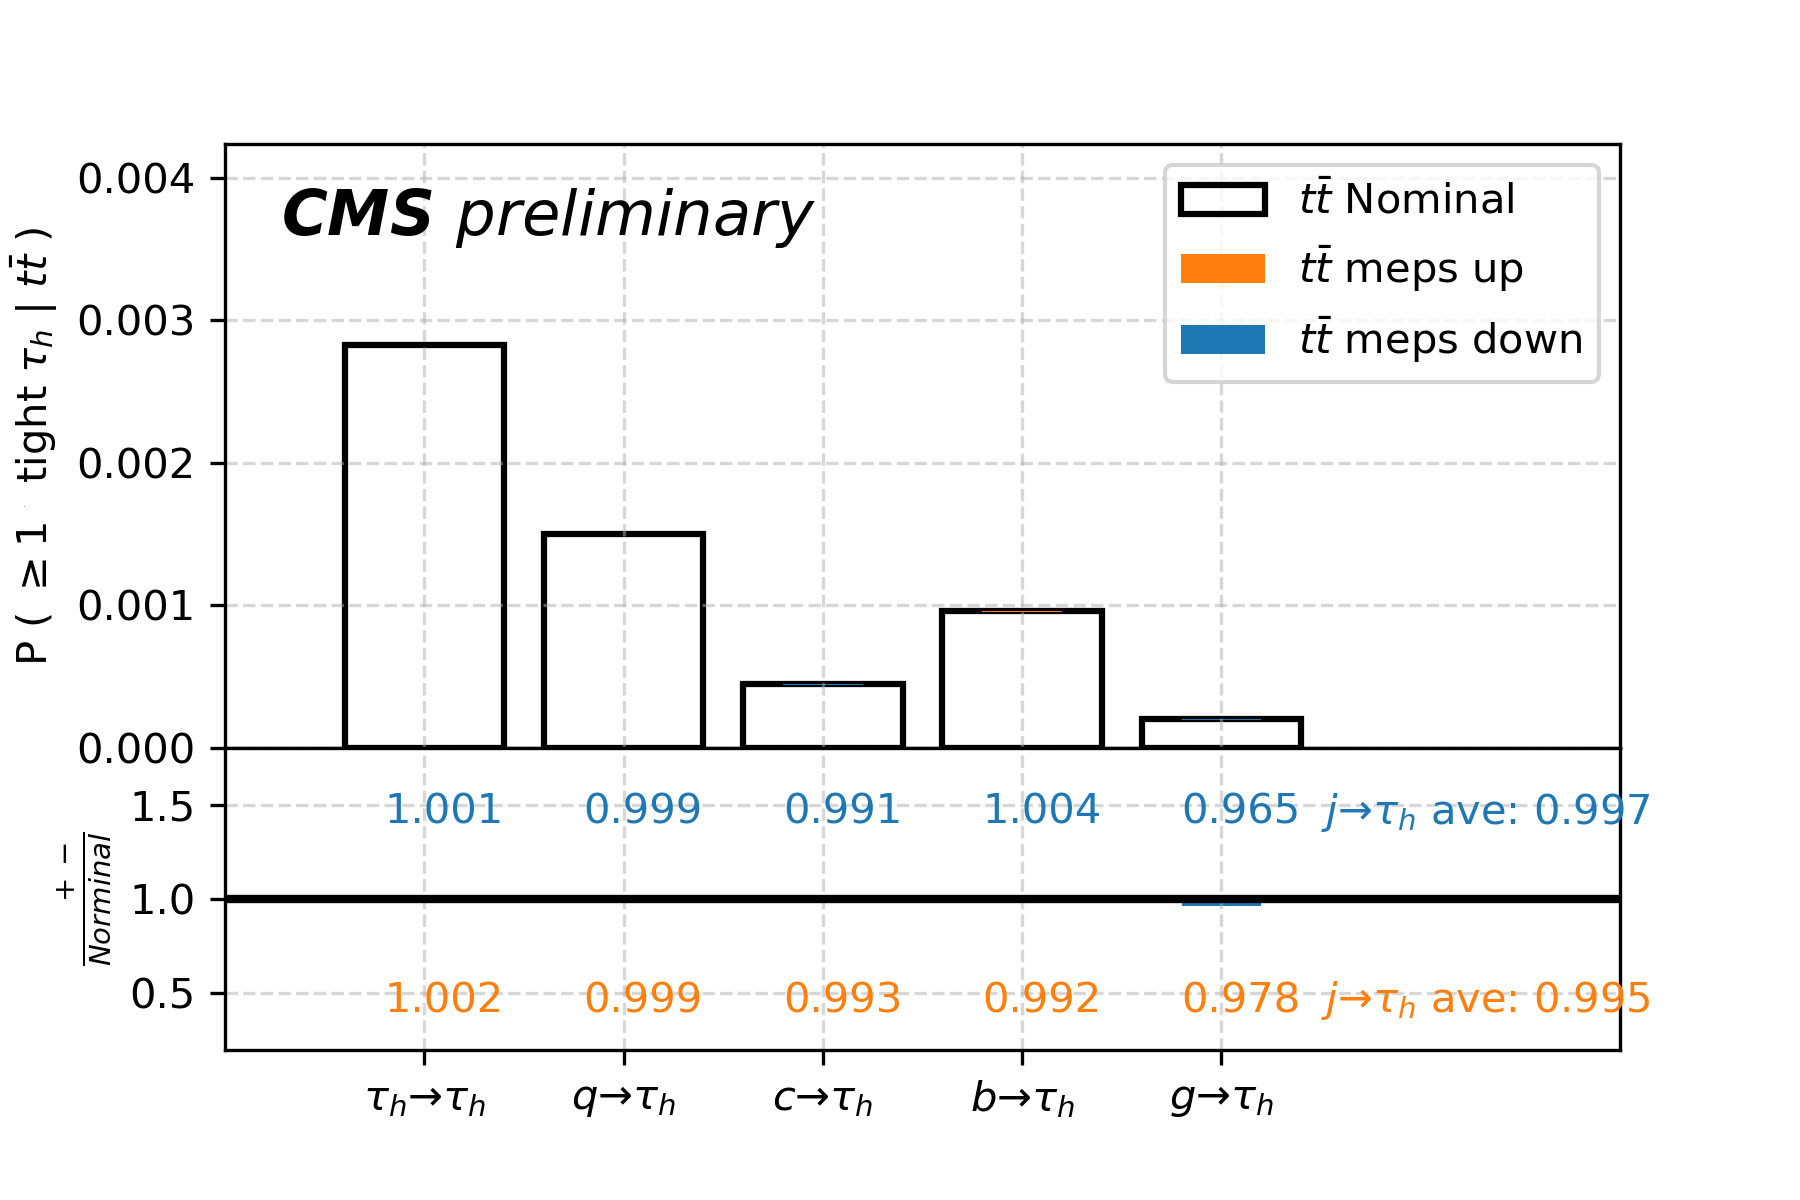
\includegraphics[width=0.49\textwidth]{chapters/Analysis/sectionSystematics/figures/ttTheoretical/2020_MCRatio_meps_tauGenFlavor_tauTight.png}
    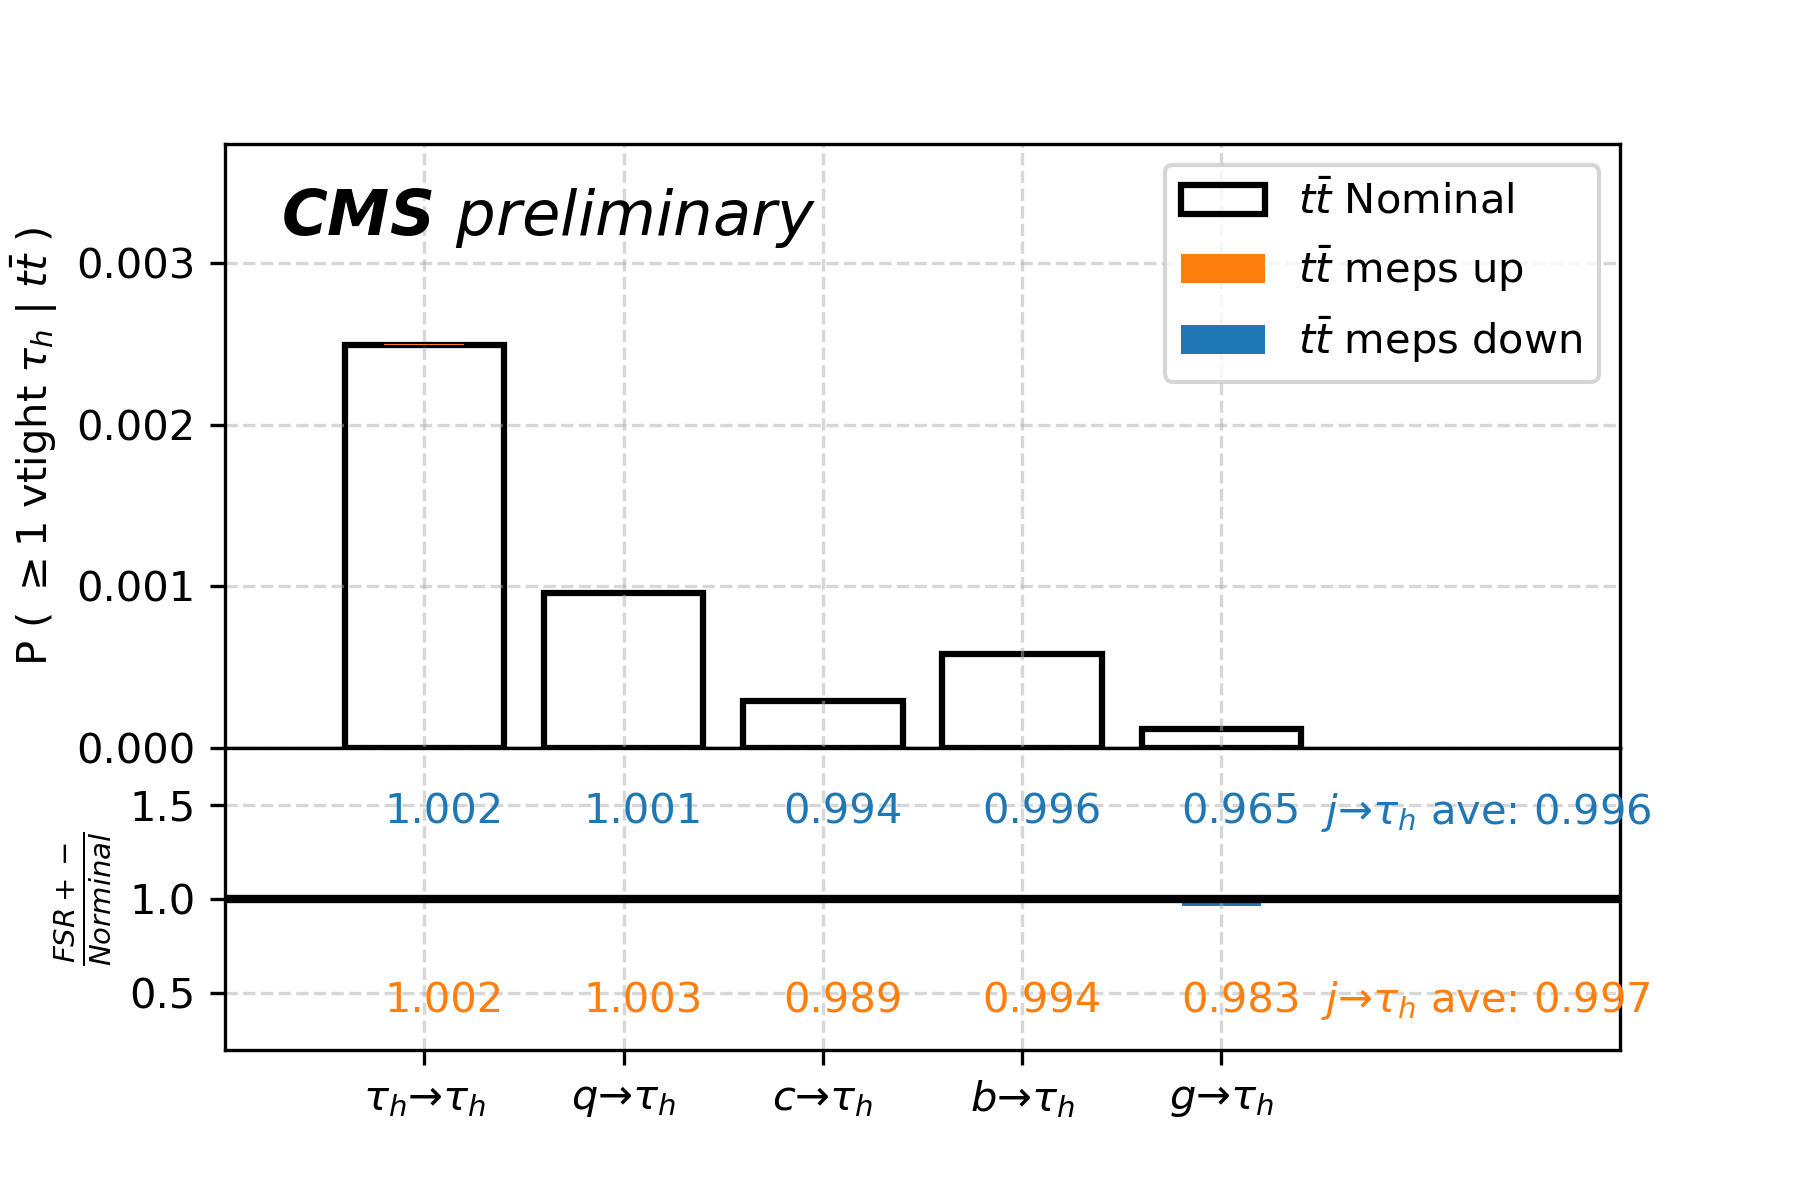
\includegraphics[width=0.49\textwidth]{chapters/Analysis/sectionSystematics/figures/ttTheoretical/2020_MCRatio_meps_tauGenFlavor_tauVTight.png}
    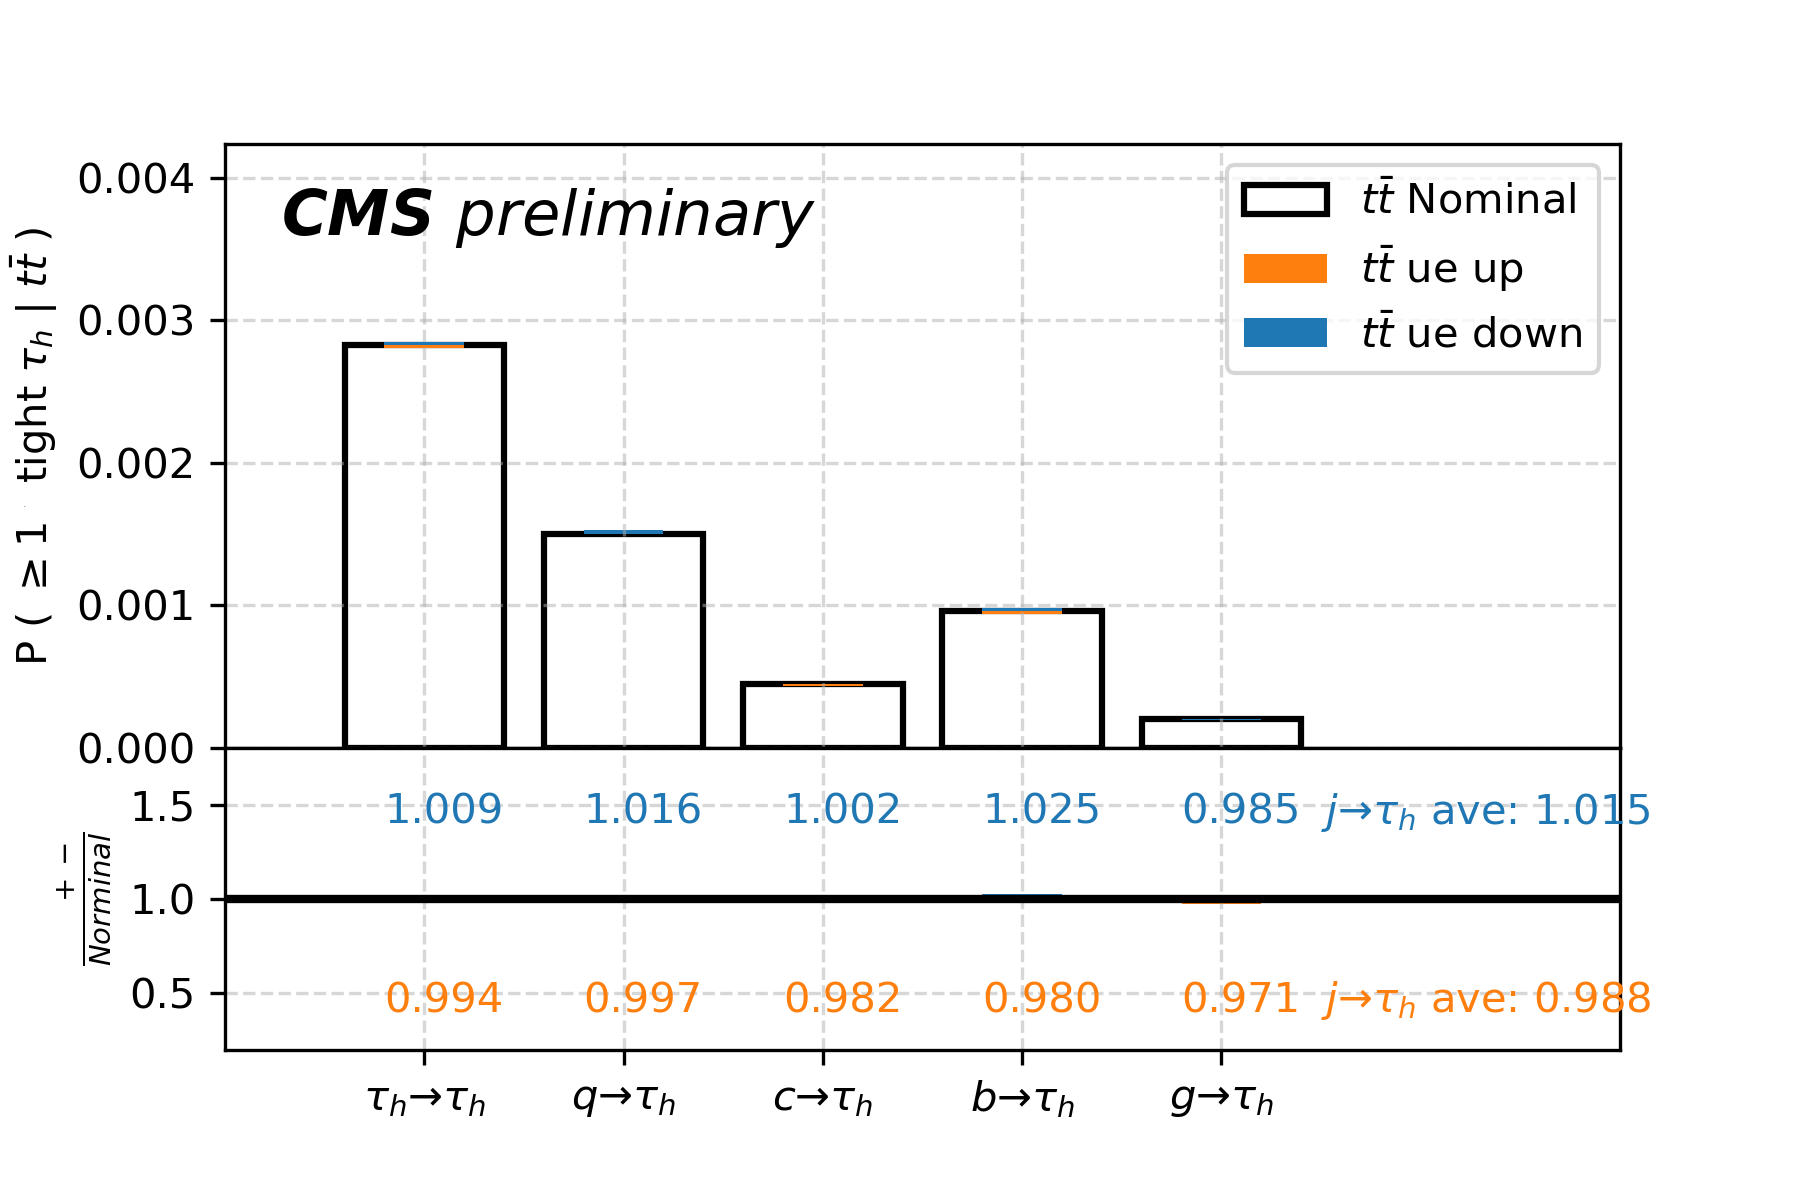
\includegraphics[width=0.49\textwidth]{chapters/Analysis/sectionSystematics/figures/ttTheoretical/2020_MCRatio_ue_tauGenFlavor_tauTight.png}
    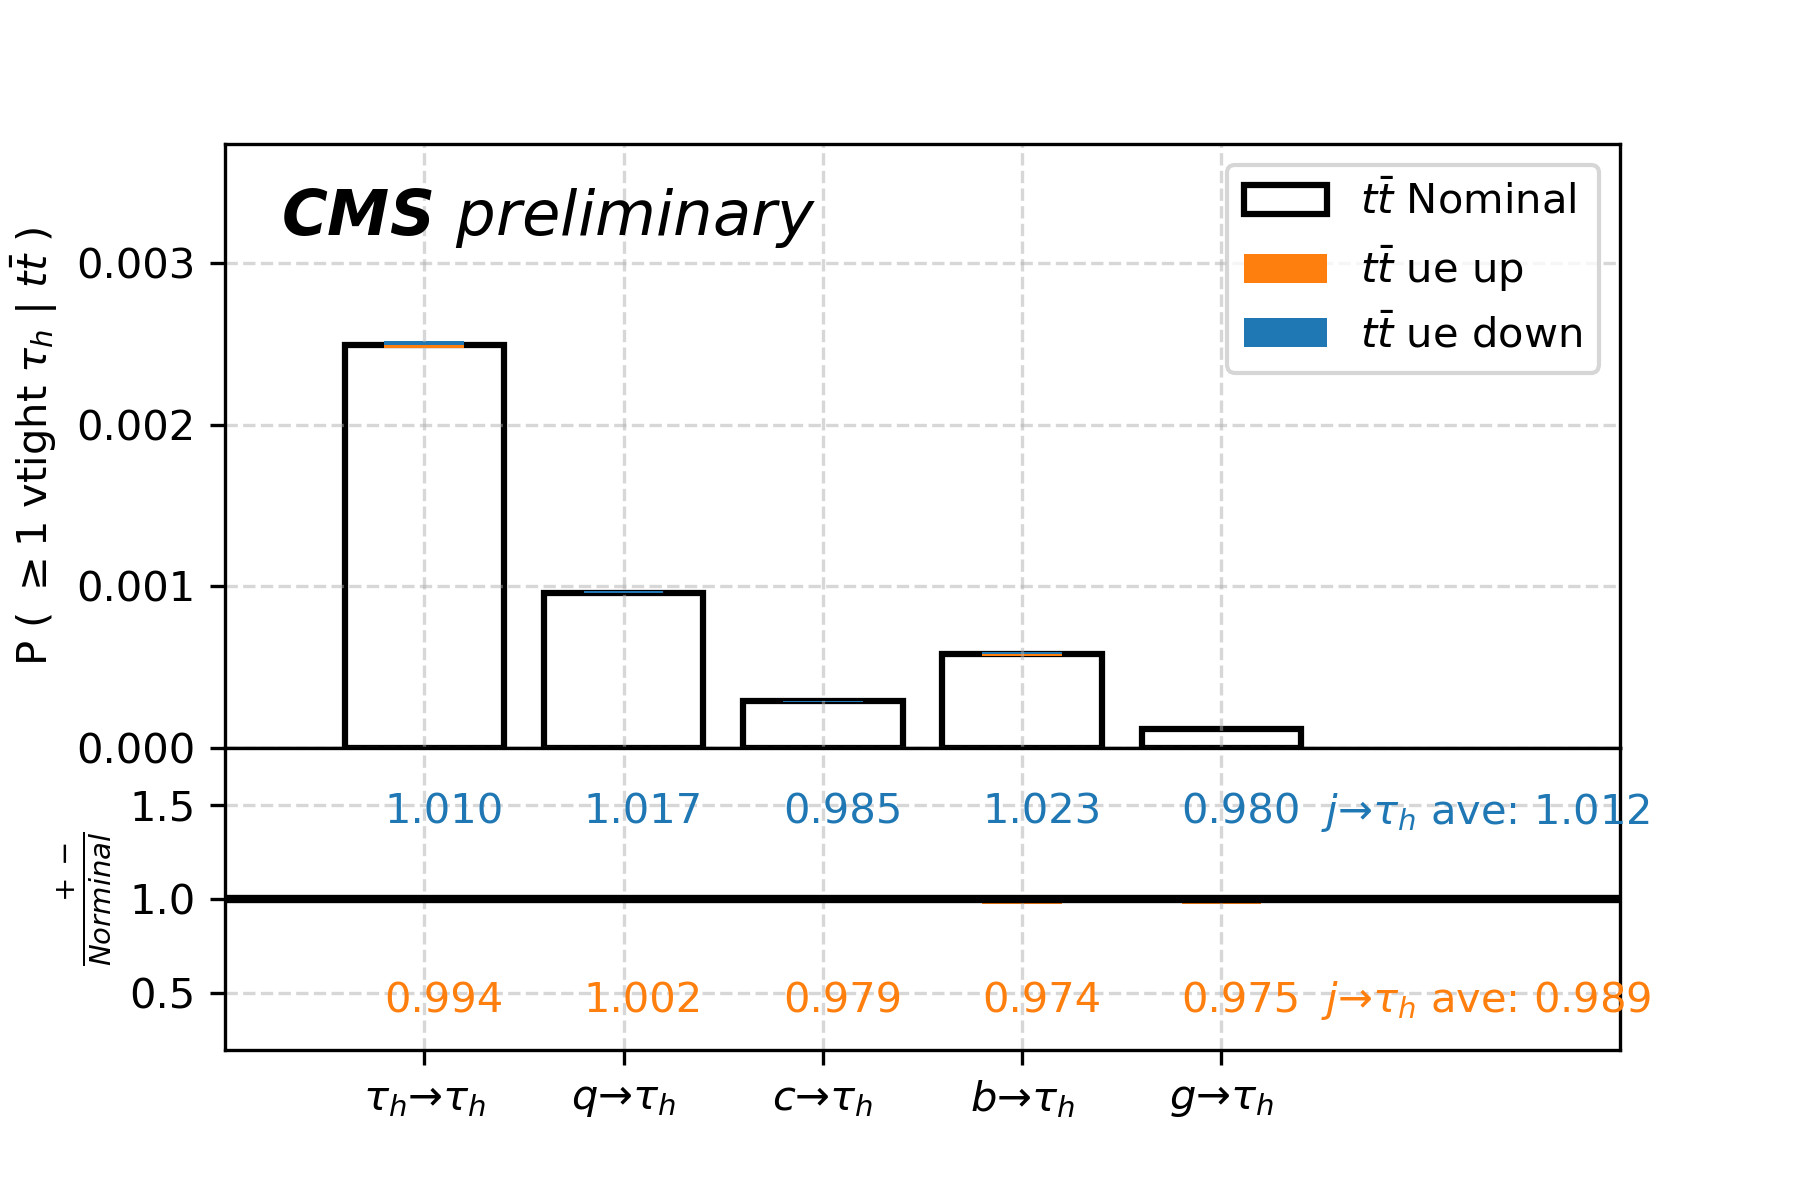
\includegraphics[width=0.49\textwidth]{chapters/Analysis/sectionSystematics/figures/ttTheoretical/2020_MCRatio_ue_tauGenFlavor_tauVTight.png}
    \caption{ISR, MEPS, UE effect on the $\PGth$ identification and $j \to \PGth$ misidentification obtained from the dedicated and the nominal \ttbar samples.
    The Tight and VTight WP are shown on the left and right, respectively.
    }
    \label{fig:analysis:systematics:sf_isr_MEPS_UE}
\end{figure}




% \begin{table}[h]
%     \centering
%     \caption{Comparison between nominal uncertainty (in a snapshot of
%         the analysis) and the uncertainty after applying the corrections
%         to the FSR variation.}
        
%     \begin{tabular}{l|cccc}
%                                   & $W\rightarrow e$ & $W\rightarrow \mu$ & $W\rightarrow \PGth$ & $W\rightarrow h$ \\
%         \hline
%         nominal                   & 1.02             & 0.71               & 2.04                & 0.40             \\
%         w/ $\PGth$ FSR corrections & 1.01             & 0.69               & 1.69                & 0.36             \\
%     \end{tabular}
%     \label{fig:fsr_correction}
% \end{table}


% Table~\label{fig:fsr_correction} shows total uncertainties of $Br(W)$ due 
% to FSR before and after the tau id and misid correction of the dedicated FSR sample.
% Before the correction, the dedicated FSR sample leads to an artificially large
% uncertainties which double counts the tau id and misid systematics.




The FSR dedicated \ttbar samples are corrected using the SF in Figure~\ref{fig:analysis:systematics:sf_fsr}.
The up and down variations given by the dedicated MC samples lead to envelops on the \ttbar event efficiencies.
As discussed in section~\ref{sec:analysis:method}, there are 21 \ttbar event efficiencies corresponding to 21 different
$\WW$ decay scenarios. For VTight WP, the 21 envelops on efficiencies due to FSR, ISR, MEPS, and UE variations are shown in 
Figure~\ref{fig:analysis:systematics:effAfterCorrFSR}-\ref{fig:analysis:systematics:effAfterCorrUE}. 
Due to the finite statistics of the dedicated MC samples, the envelops edges are smeared by the MC statistics, 
which are also shown in the Figure~\ref{fig:analysis:systematics:effAfterCorrFSR} - \ref{fig:analysis:systematics:effAfterCorrUE}.


\begin{figure}
    \centering
    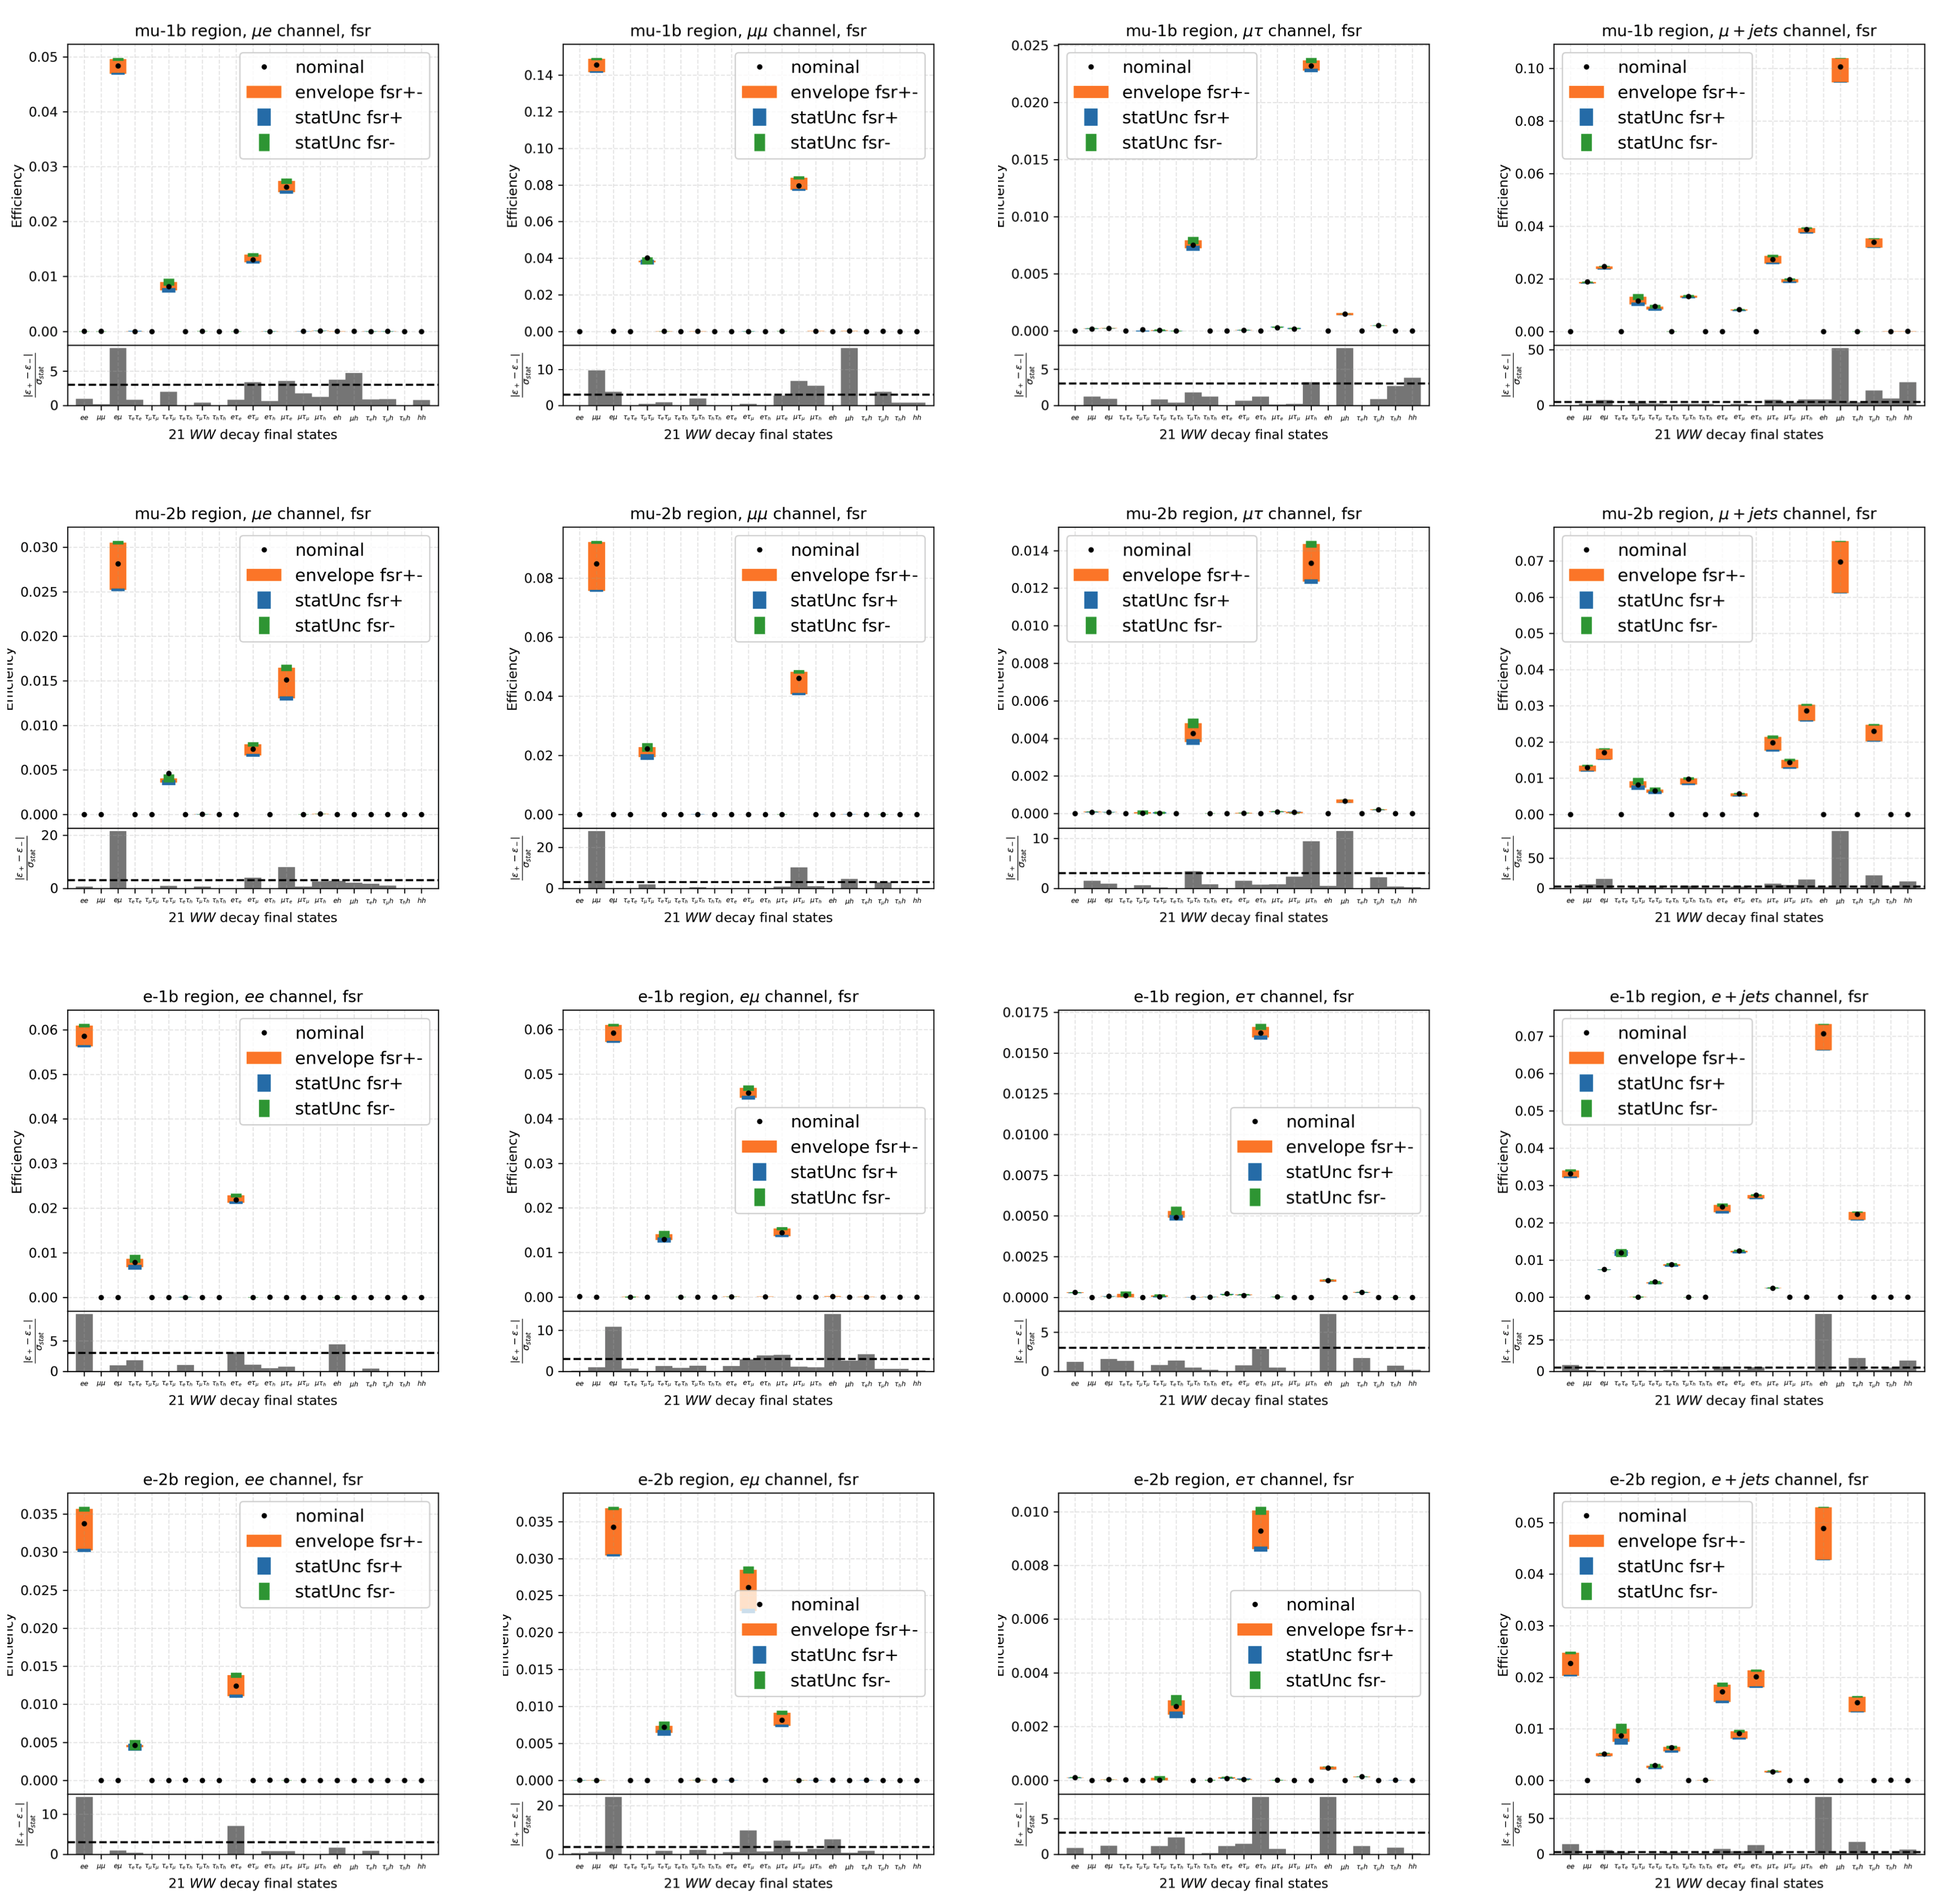
\includegraphics[width=0.99\textwidth]{chapters/Analysis/sectionSystematics/figures/ttTheoretical/fsr.png}    
    \caption{envelops on 21 efficiencies due to final state radiation (FSR) uncertainty. VTight WP is shown.}
    \label{fig:analysis:systematics:effAfterCorrFSR}
\end{figure}



\begin{figure}
    \centering
    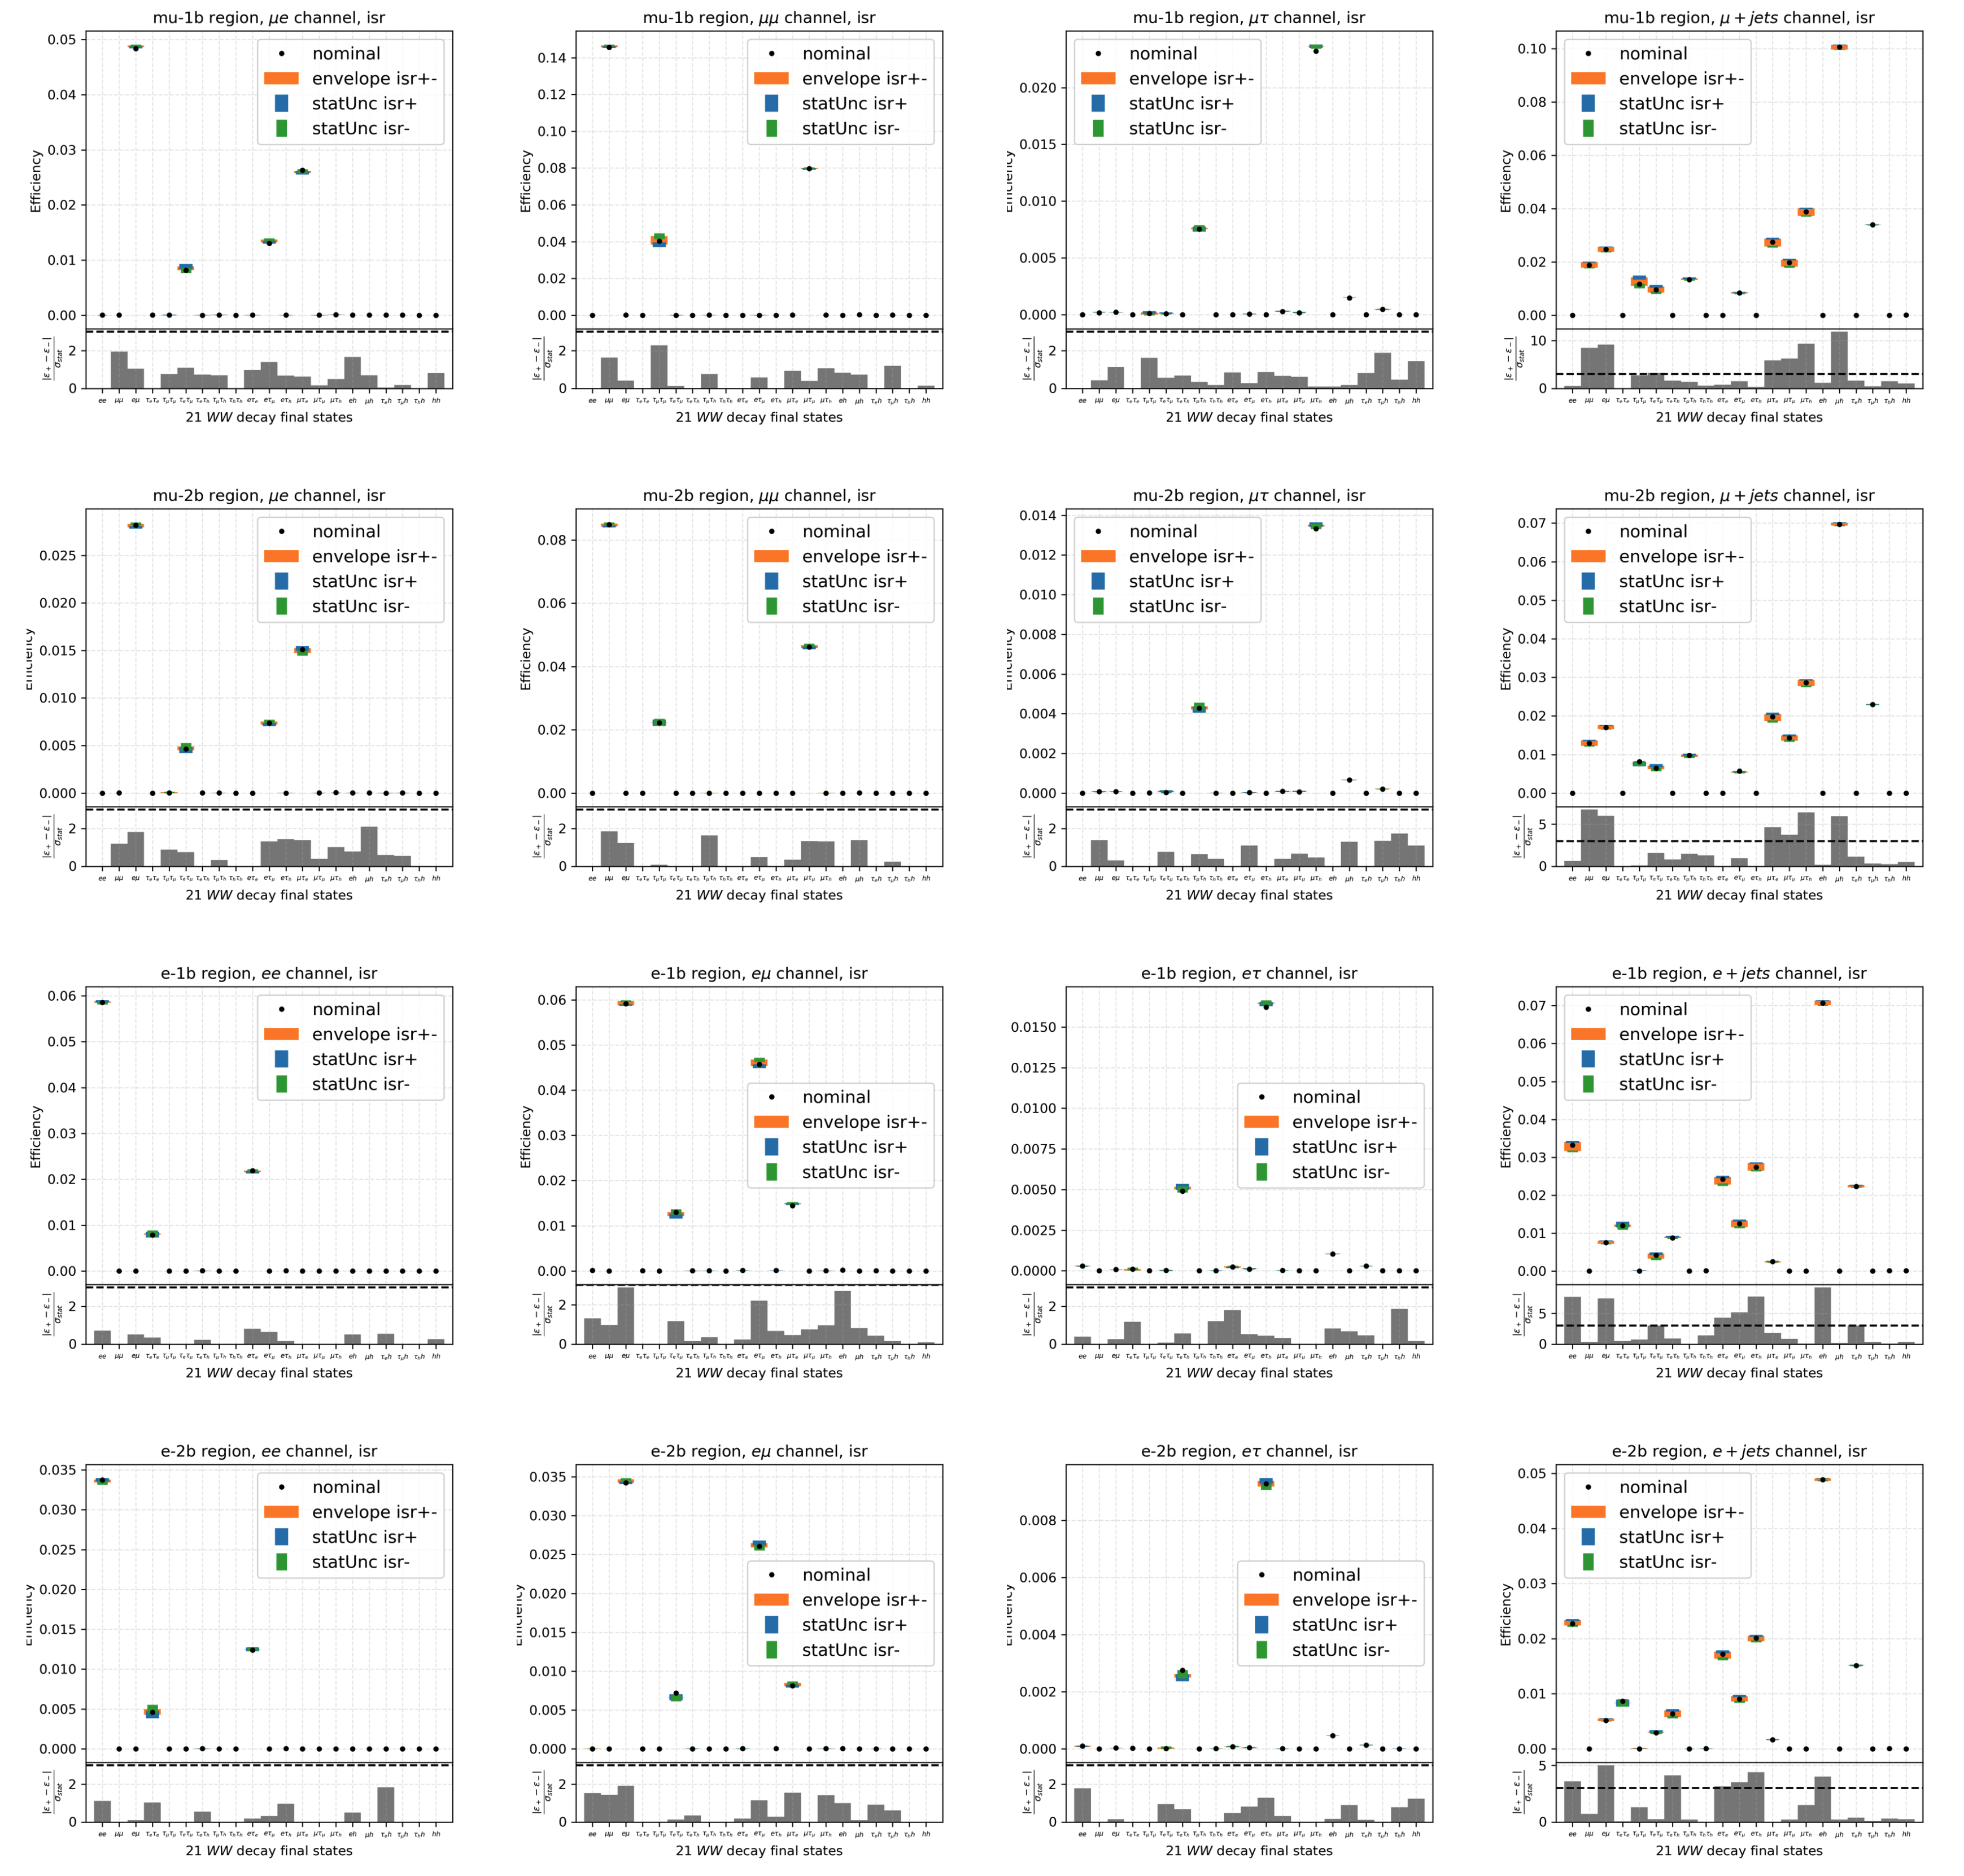
\includegraphics[width=0.99\textwidth]{chapters/Analysis/sectionSystematics/figures/ttTheoretical/isr.png}
    \caption{Envelops on 21 efficiencies due to initial state radiation (ISR) uncertainty. VTight WP is shown.}
    \label{fig:analysis:systematics:effAfterCorrISR}
\end{figure}


\begin{figure}
    \centering
    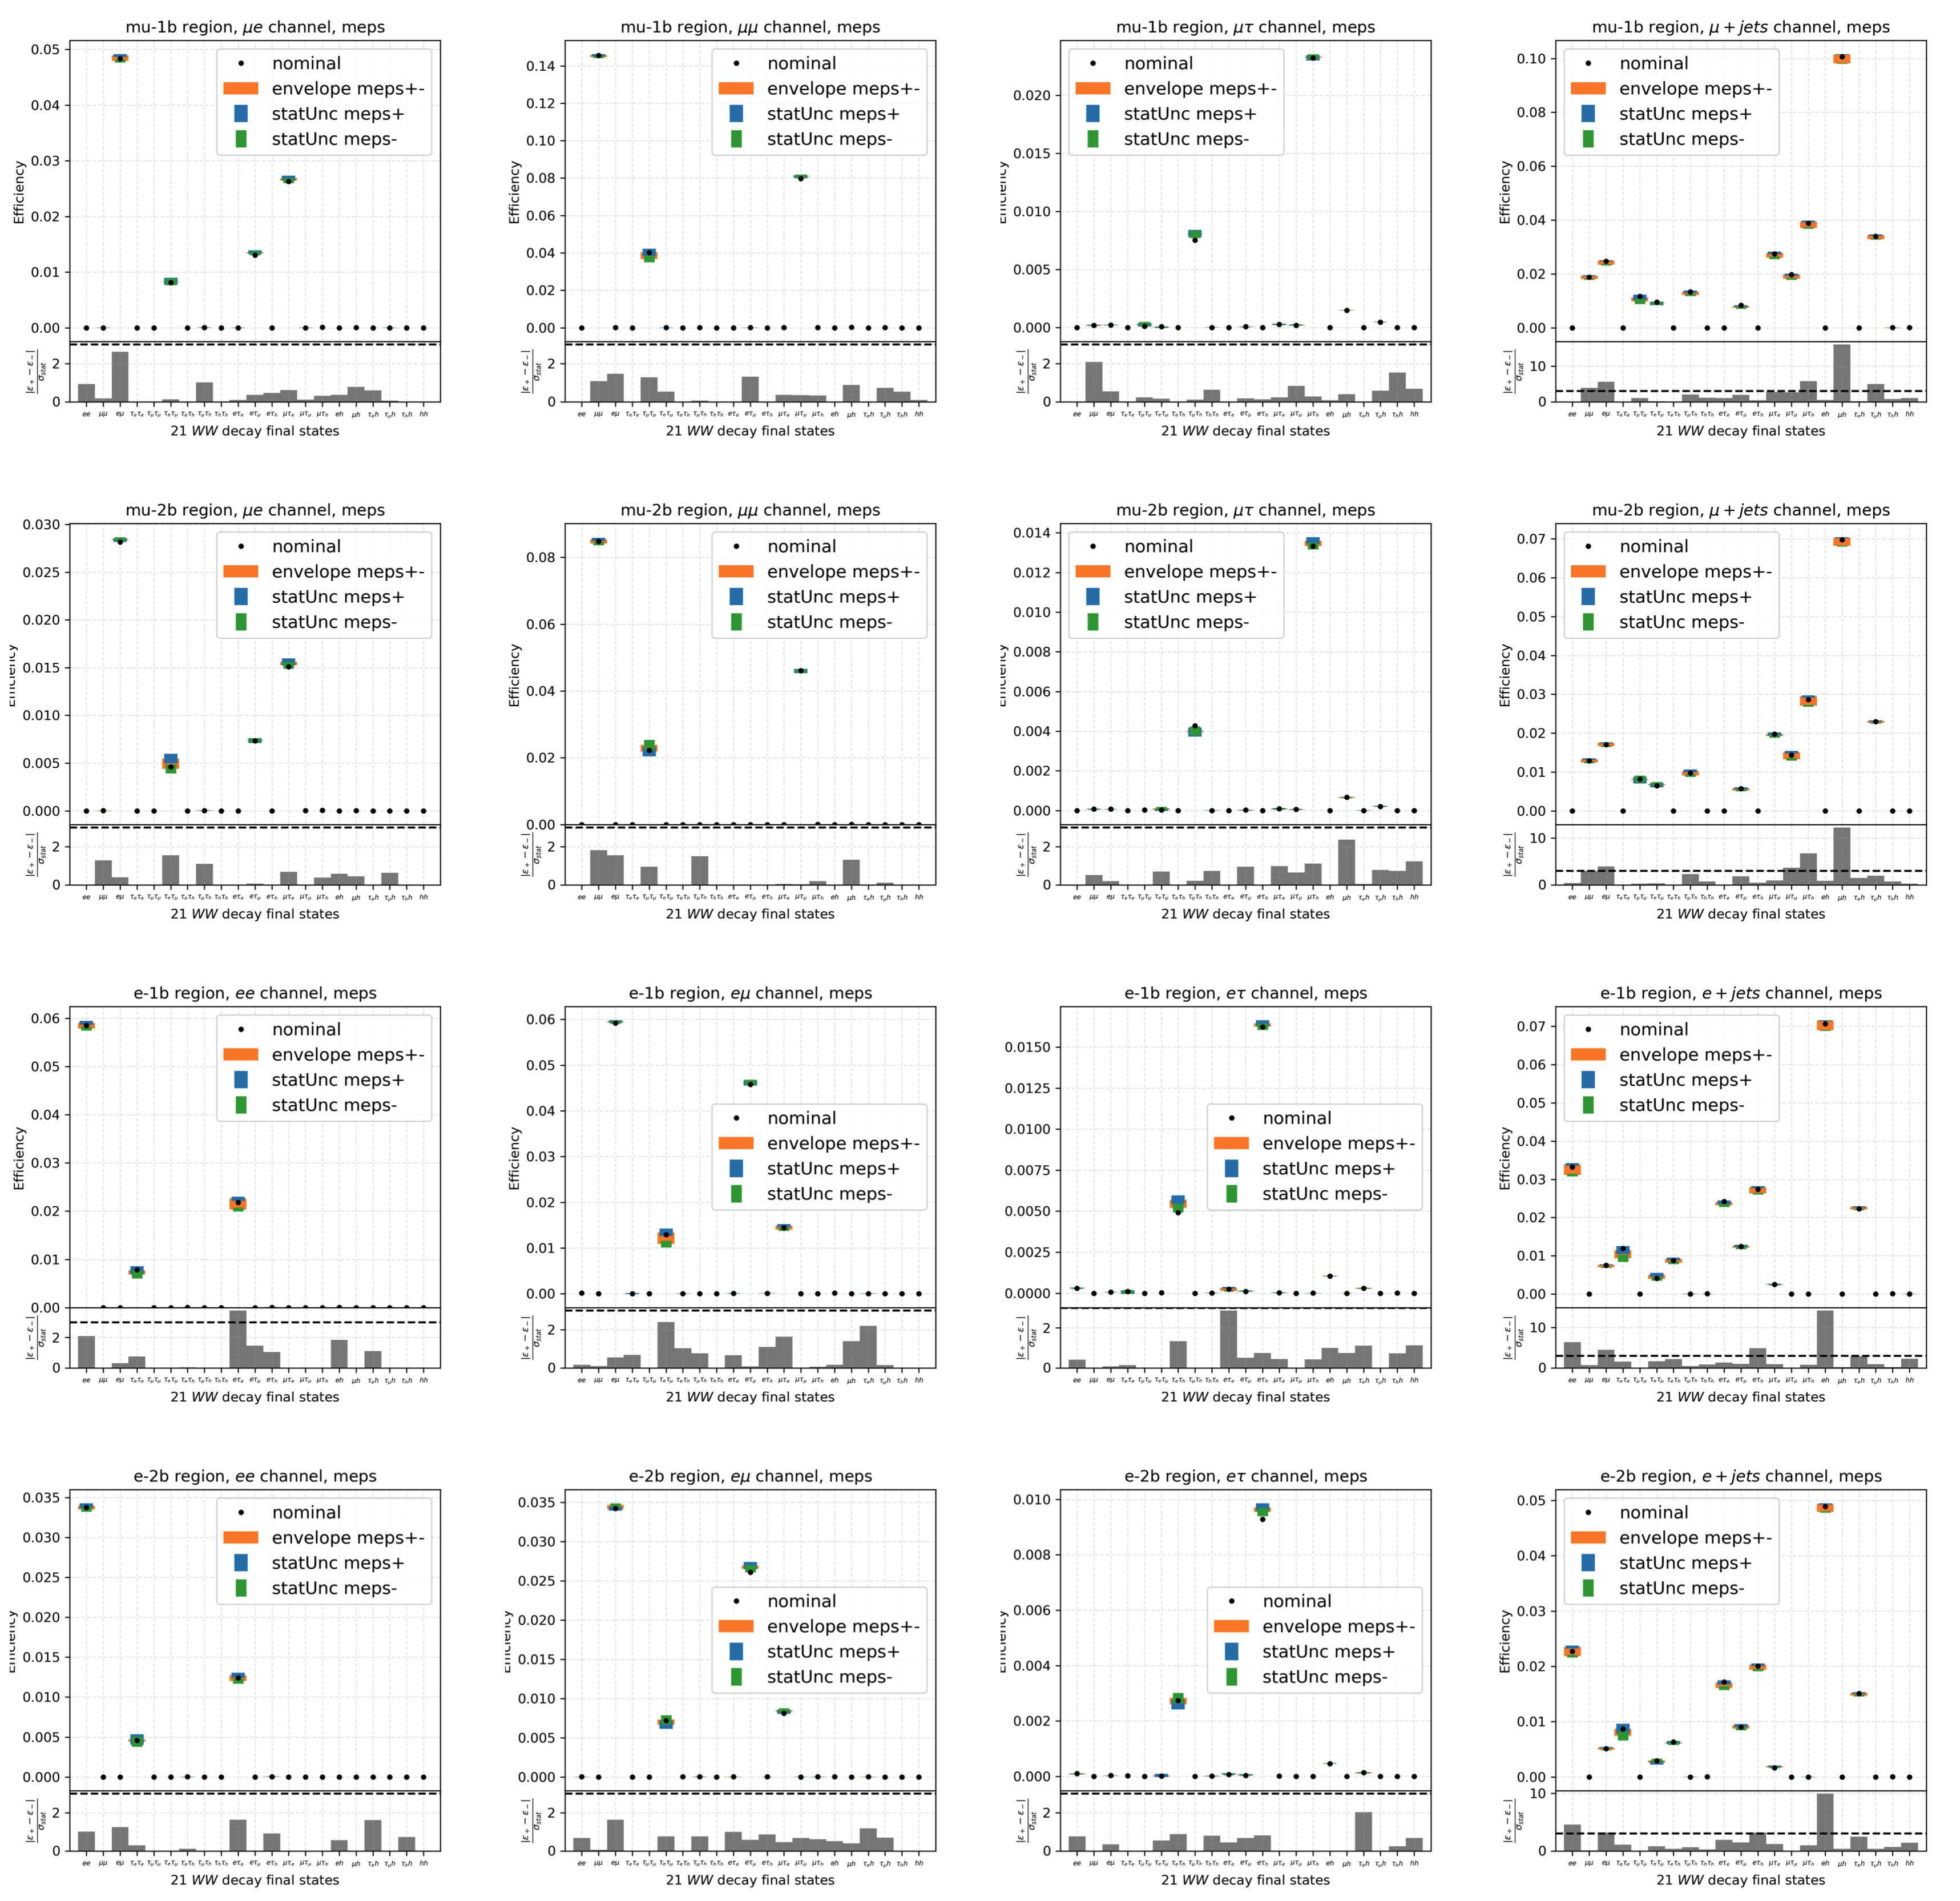
\includegraphics[width=0.99\textwidth]{chapters/Analysis/sectionSystematics/figures/ttTheoretical/meps.png}
    \caption{Envelops on 21 efficiencies due to parton shower matching (ME-PS) uncertainty. VTight WP is shown.}
    \label{fig:analysis:systematics:effAfterCorrMEPS}
\end{figure}


\begin{figure}
    \centering
    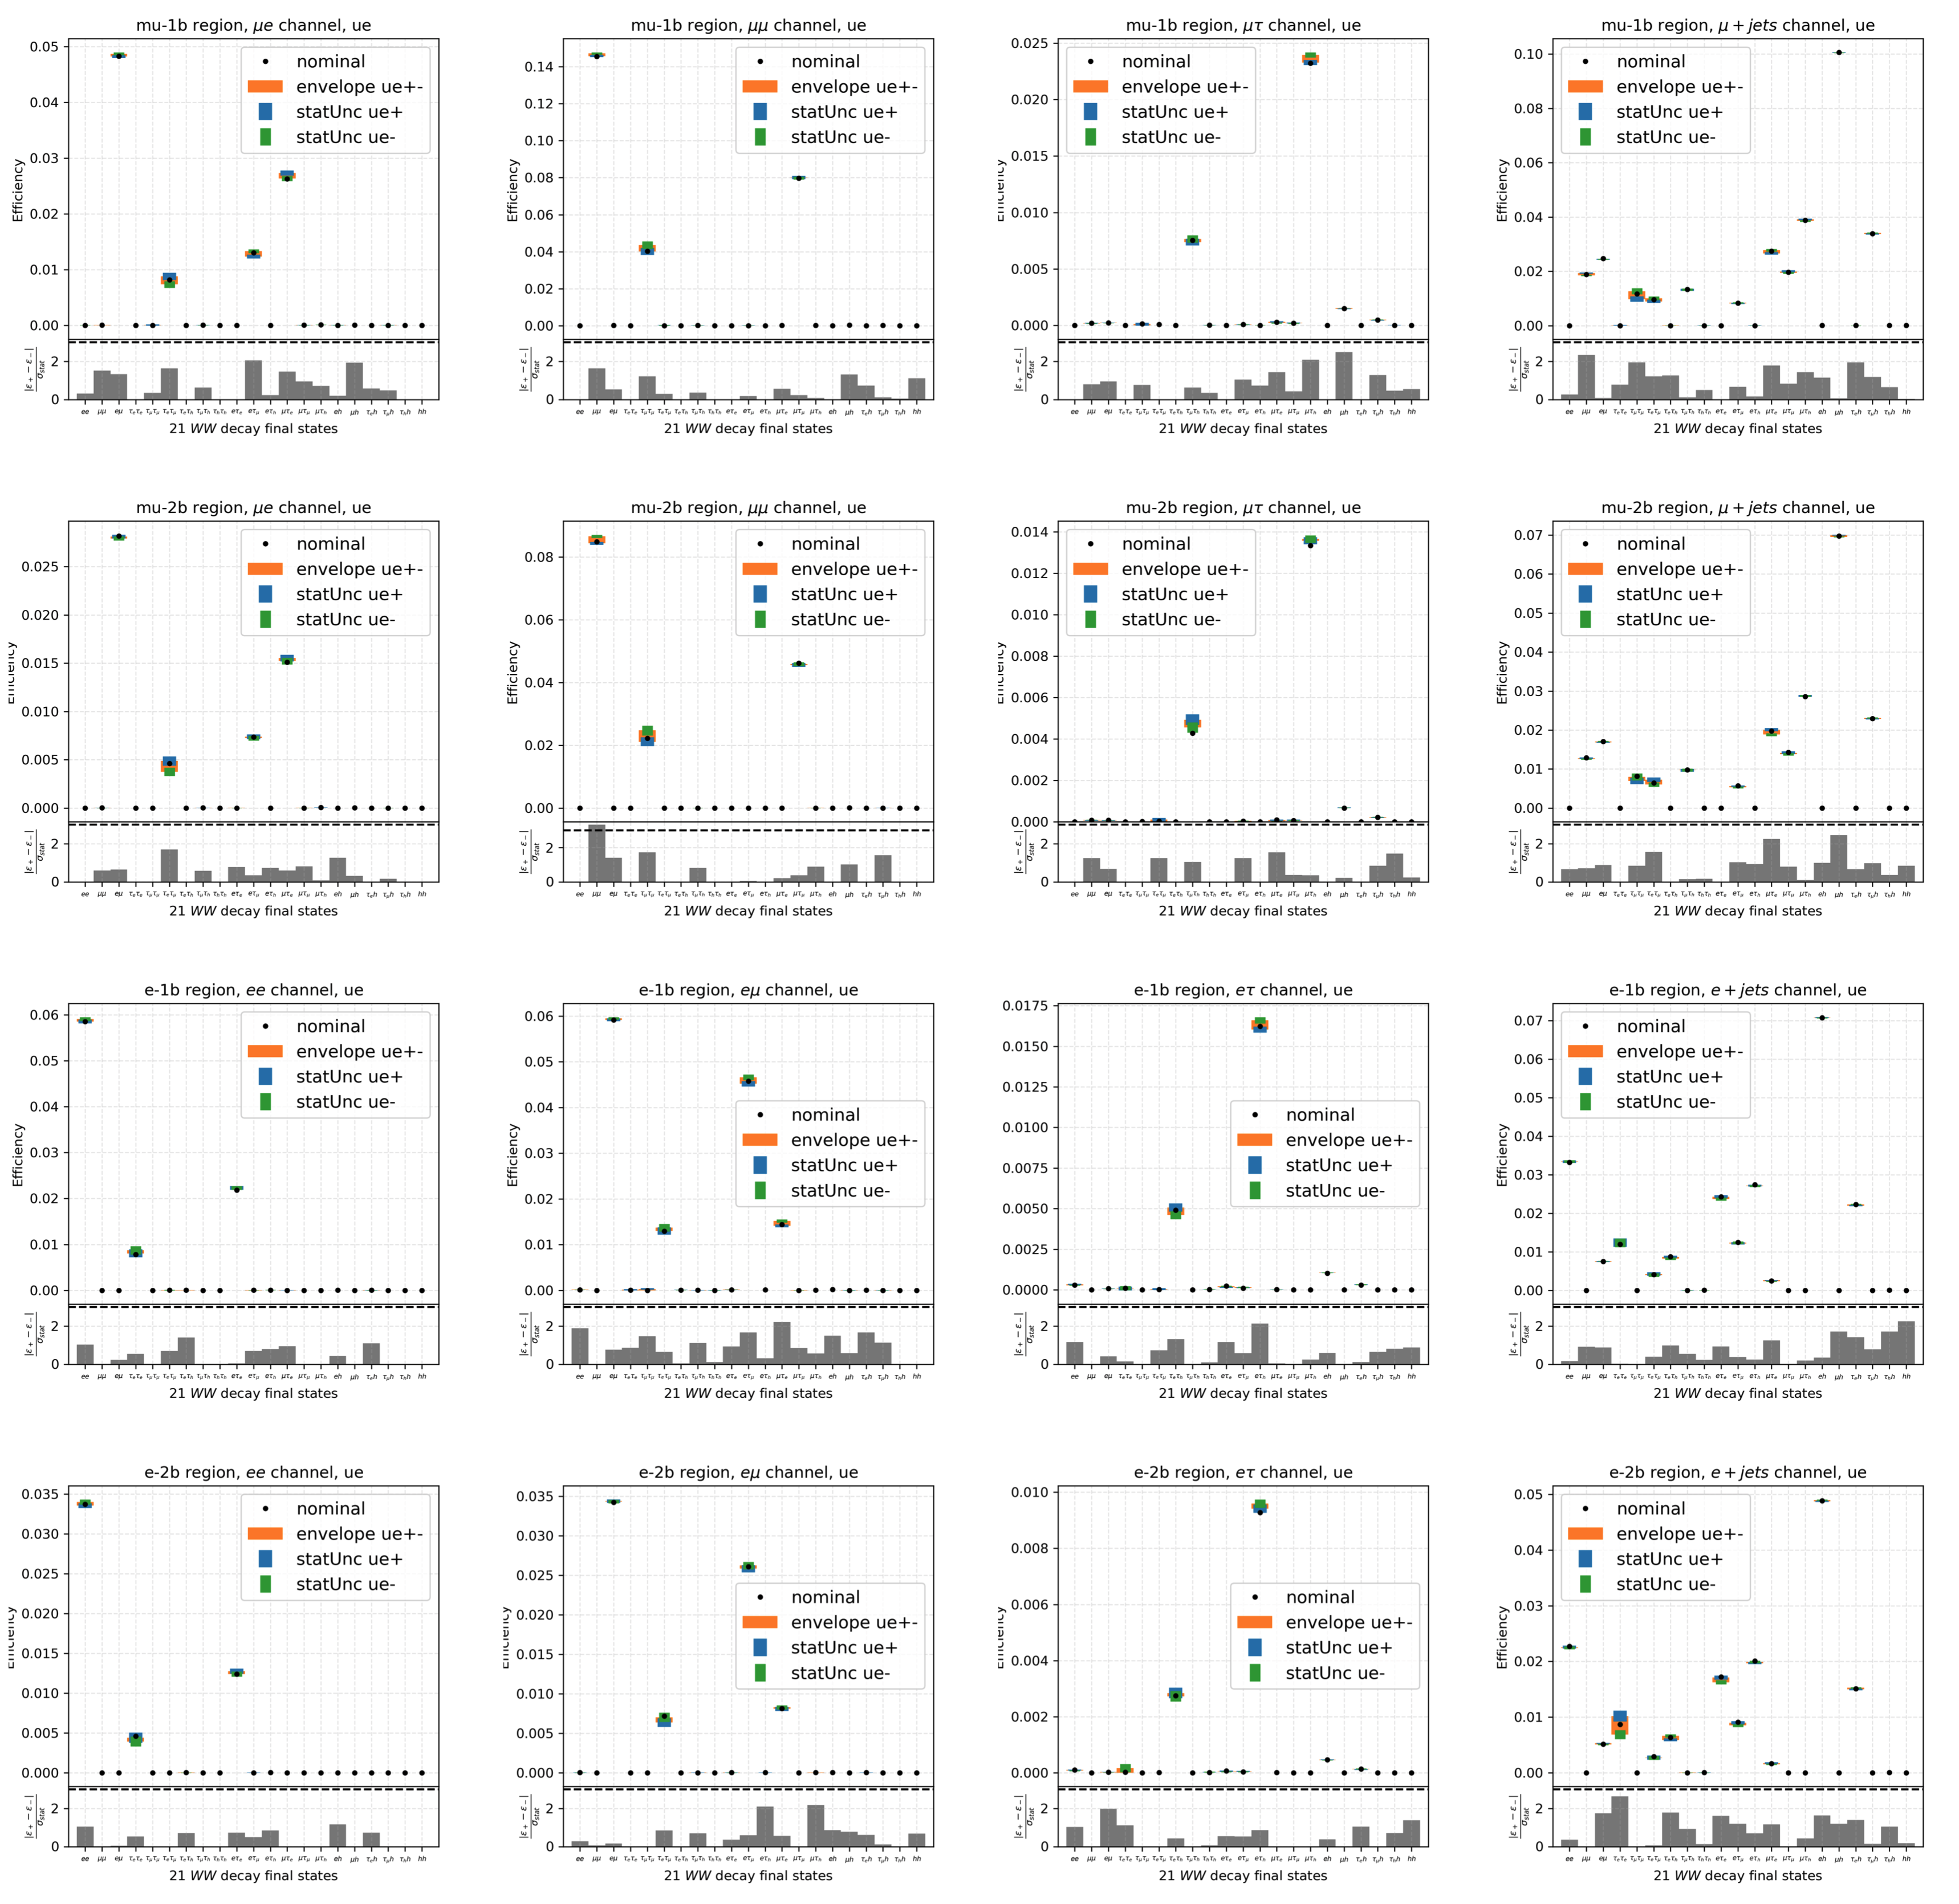
\includegraphics[width=0.99\textwidth]{chapters/Analysis/sectionSystematics/figures/ttTheoretical/ue.png}
    \caption{Envelops on 21 efficiencies due to underline event (UE) uncertainty. VTight WP is shown.}
    \label{fig:analysis:systematics:effAfterCorrUE}
\end{figure}




% \subsubsection{Tau Hadronic Decay Reweighting}

% The tau decay in the simulation is handled by \PYTHIA using the \PYTHIA default branching fractions, which are about 0.5\% different from the experimental values in the PDG~\ref{pdg2020}. This deviation is corrected by reweighting the simulated events with hadronic taus to match the PDG tau decay branching fractions. The 


% The MC events with $\PGth$ in the \cet and $\mu \PGth$ channel is essential to the sensitivity of the $Br(W\to\PGth)$ measurement. However, the tau's hadronic decay branching fraction $B(\PGth \to  \rm{hadrons})$ in the MC simulation are different from the experimental world average in the PDG. The $\PGth$ selection efficiency could be impacted by such difference because various tau's hadronic  decay mode have different efficiencies in the CMS $\PGth$ reconstruction with SPH algorithm.

% Thus it is necessary to reweight the MC events to correct the deviation of tau's decay in the simulation with respect to the PDG values. For the values in the \PYTHIA simulation assumption and the PDG world average, tau's hadronic decay branching fractions are listed in table~\ref{tab:tauhReweighting}. The difference between values in \PYTHIA8 and PDG is about $0.5\%$. The ratios of PDG and \PYTHIA values are also included, which are the event weights applied for the $\PGth \to h$ reweighting.

    
    
% \begin{table}[ht]
%   \centering
%   \setlength{\tabcolsep}{1 em}
%   \renewcommand{\arraystretch}{1.5}
%   \caption{ The values of $B(\PGth \to  \rm{hadrons})$ in PYTHIA8 and in PDG.}
%   \begin{tabular}{l|c|c|c}
%   \hline
%                               & PDG        & \PYTHIA   & PDG / \PYTHIA \\
%   \hline
%   $B(\PGth\to \PGp^\pm)$       & 0.1082(5)  & 0.1076825 & 1.00481       \\
%   $B(\PGth\to \PGp^\pm+ \PGp^0)$& 0.2549(9)  & 0.2537447 & 1.00455       \\
%   $B(\PGth\to \PGp^\pm+2\PGp^0)$& 0.0926(10) & 0.0924697 & 1.00141       \\
%   $B(\PGth\to3\PGp^\pm)$       & 0.0931(5)  & 0.0925691 & 1.00574       \\
%   $B(\PGth\to3\PGp^\pm+ \PGp^0)$& 0.0462(5)  & 0.0459365 & 1.00574       \\
%   \hline
%   \end{tabular}
%   \label{tab:analysis:calibration:tauhReweighting}
% \end{table}


% \begin{figure}
%     \centering
%     \includegraphics[width=0.99\textwidth]{chapters/Analysis/sectionCalibration/figures/tauBr/tauhDecay_mutau.png}
%     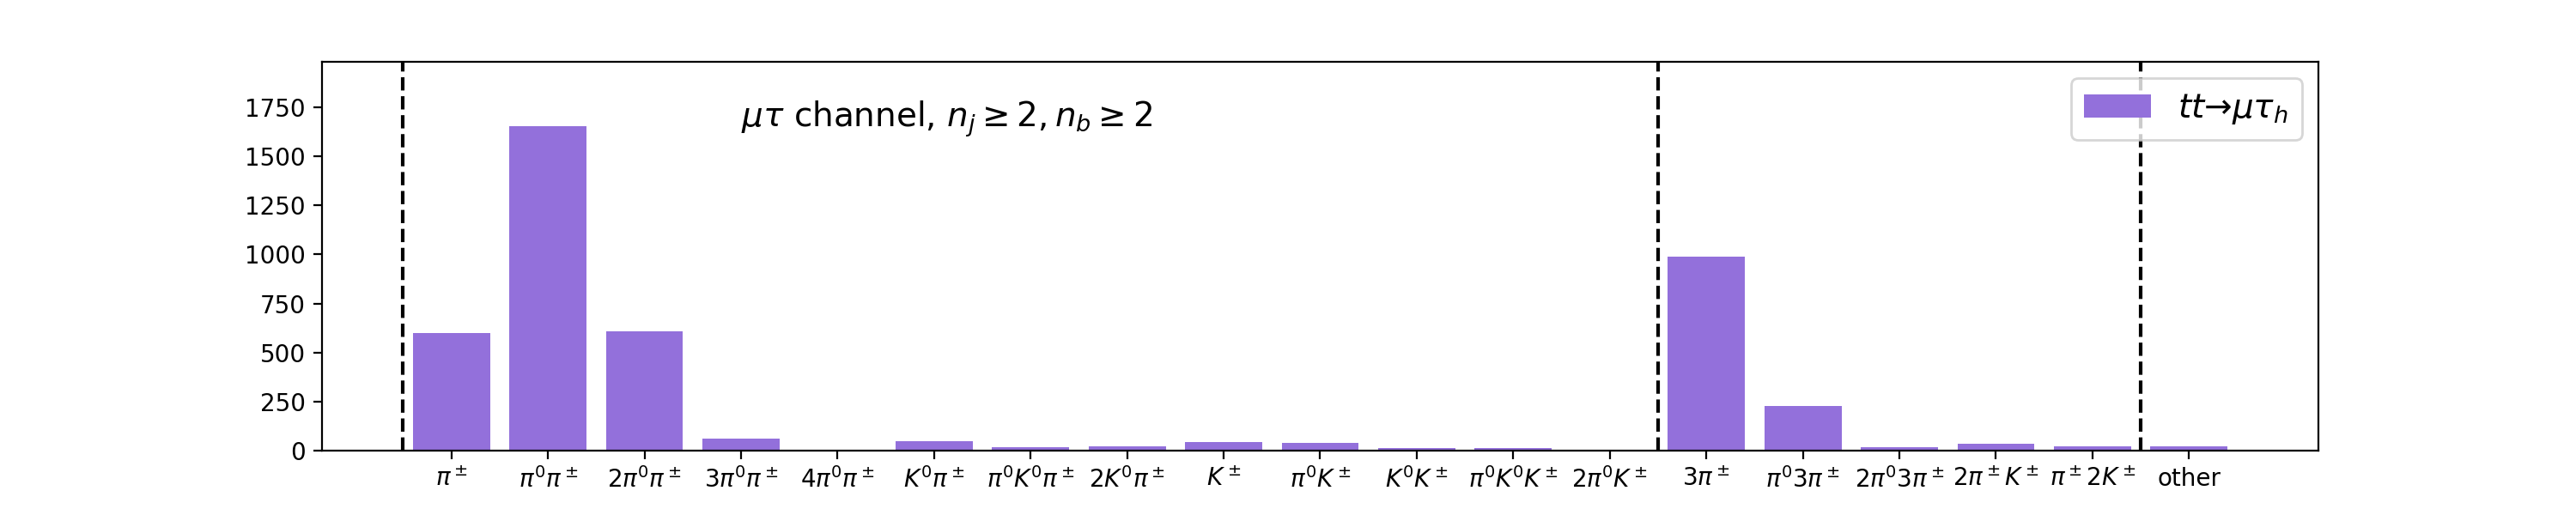
\includegraphics[width=0.99\textwidth]{chapters/Analysis/sectionCalibration/figures/tauBr/tauhDecay_mutau2.png}
%     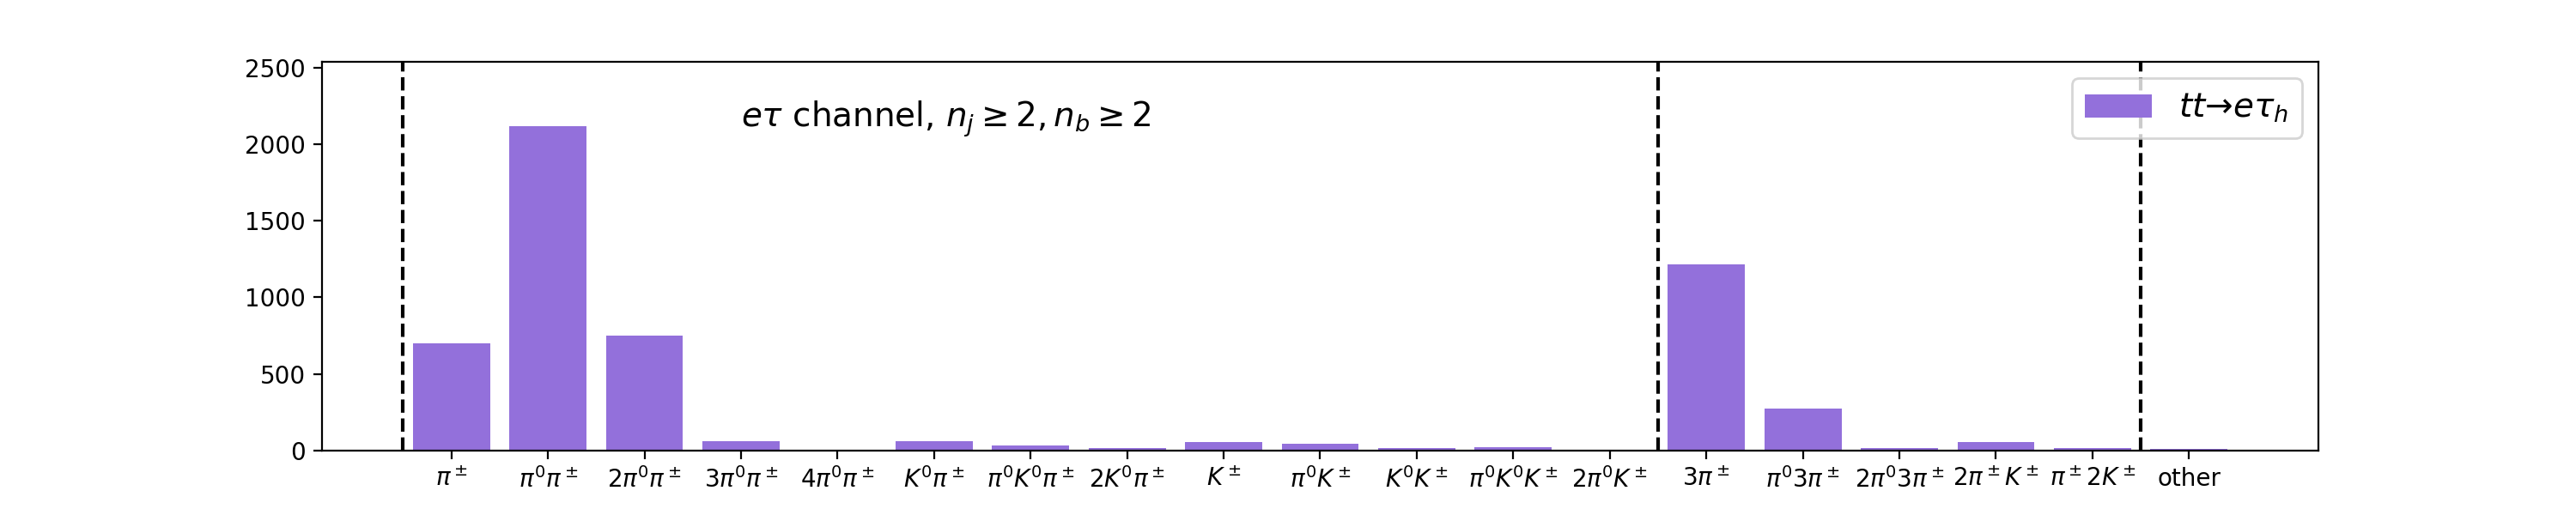
\includegraphics[width=0.99\textwidth]{chapters/Analysis/sectionCalibration/figures/tauBr/tauhDecay_etau.png}
%     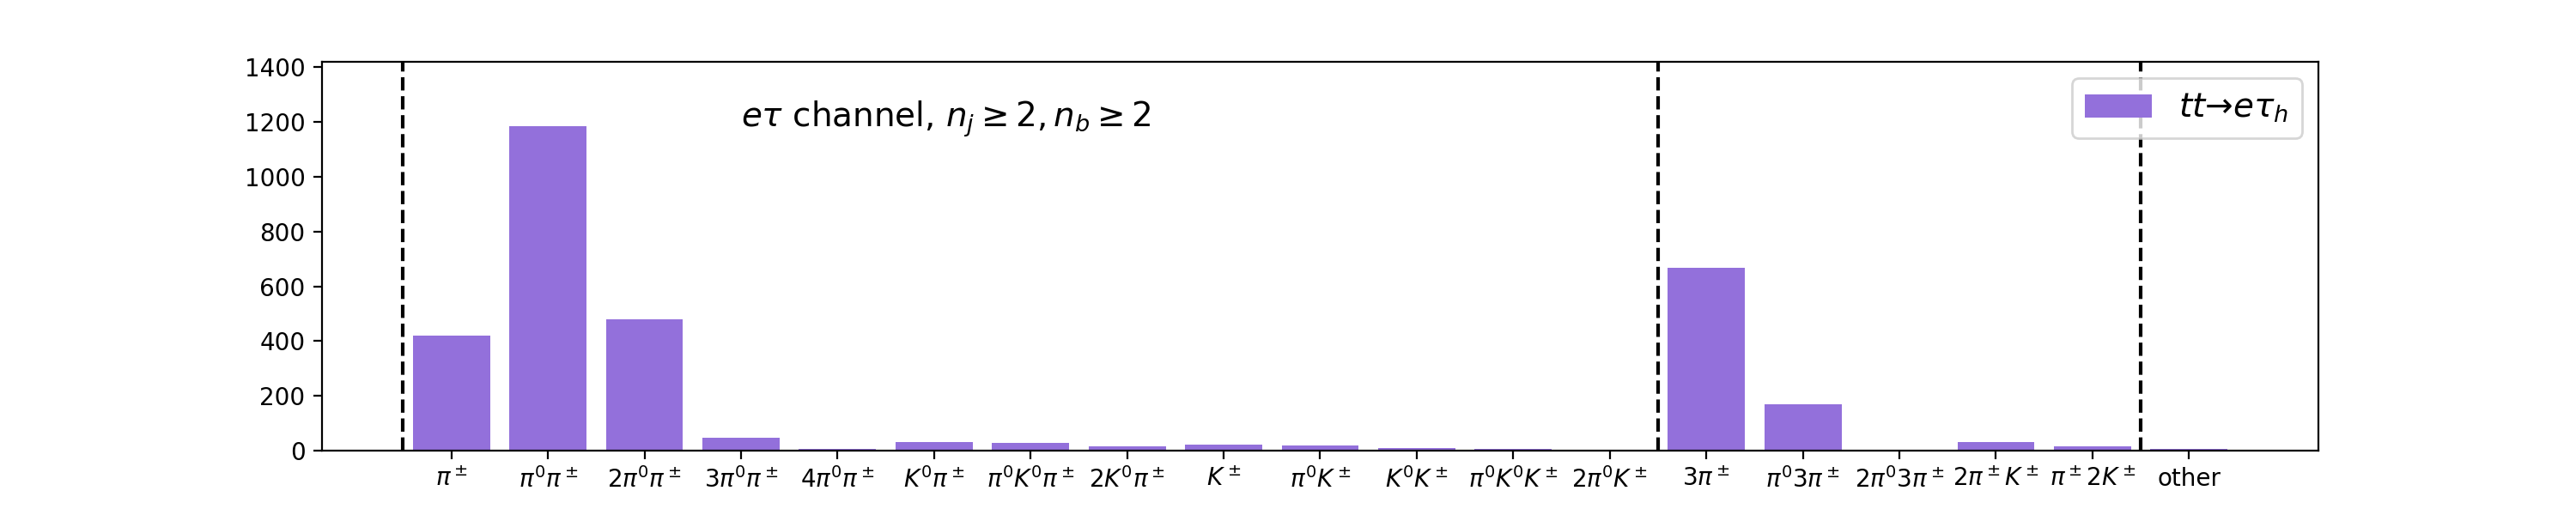
\includegraphics[width=0.99\textwidth]{chapters/Analysis/sectionCalibration/figures/tauBr/tauhDecay_etau2.png}
%     \caption{The gen-level daughter mesons from hadronicly decaying taus in the $tt\to \mu \PGth, e \PGth$ events passing $\mu \PGth$ and $e \PGth$ selection.}
%     \label{fig:appendix:reweightTauhBr:tauhBr}
% \end{figure}


% In MC events, the gen-level daughter mesons from hadronically decaying taus are saved.  The $\PGth$'s daughter mesons in the $tt\to \mu \PGth, e \PGth$ events  passing $\mu \PGth$ and $e \PGth$ selection are shown in Figure~\ref{fig:appendix:reweightTauhBr:tauhBr} The leading contributions to the reconstructed $\PGth$ are $\PGth\to \PGp^\pm+\PGp^0 $, $\PGth\to 3\PGp^\pm$, $\PGth\to \PGp^\pm+2\PGp^0$, $\PGth\to \PGp^\pm$, $\PGth\to 3\PGp^\pm + \PGp^0$.  MC events with taus in those five decay modes are reweighted by 

% \begin{equation}
%   w = \frac{^{\rm PDG} B(\PGth \to  \rm{hadrons}) }{^{\rm \PYTHIA} B( \PGth \to \rm{hadrons} )}. 
% \end{equation} 


% \noindent The uncertainties of the weights are from the the PDG uncertainties.  The systematic uncertainty due to the uncertainties of $B(\PGth \to  \rm{hadrons})$ reweighting can be estimated. The effect of the $B(\PGth \to  \rm{hadrons})$  reweighting on the $B(W)$ result is small. The relative systematics from $B(\PGth \to  \rm{hadrons})$ reweighting are about $0.003 - 0.146 \%$,  shown in table~ \ref{tab:syst_tauhReweighting}.


\FloatBarrier



\subsection{Shape Analysis}

As described previously, each source of uncertainty is accounted for in
the shape analysis by including one or more associated nuisance
parameters.  After minimizing the likelihood, post-fit values for the
nuisance parameters and their associated uncertainties are obtained.
This is illustrated in Figure~\ref{fig:analysis:systematics:pulls_all}.  In general, the
pulls on the nuisance parameters do not exceed two standard deviations of their
initial uncertainty, but many of the nuisance parameters do become
constrained.  Additionally, the correlations for each parameter can be
obtained and are displayed in Figure~\ref{fig:analysis:systematics:corr_matrix}.  In order to
isolate the effect of each nuisance parameter on the uncertainty of the 
branching fractions, the minimization is repeated while individually fixing each
nuisance parameter either to its post-fit value plus or minus the
post-fit uncertainty.  The result of this process is shown in
Figure~\ref{fig:analysis:systematics:pulls_all}.

\begin{sidewaysfigure}[ht]
    \centering
    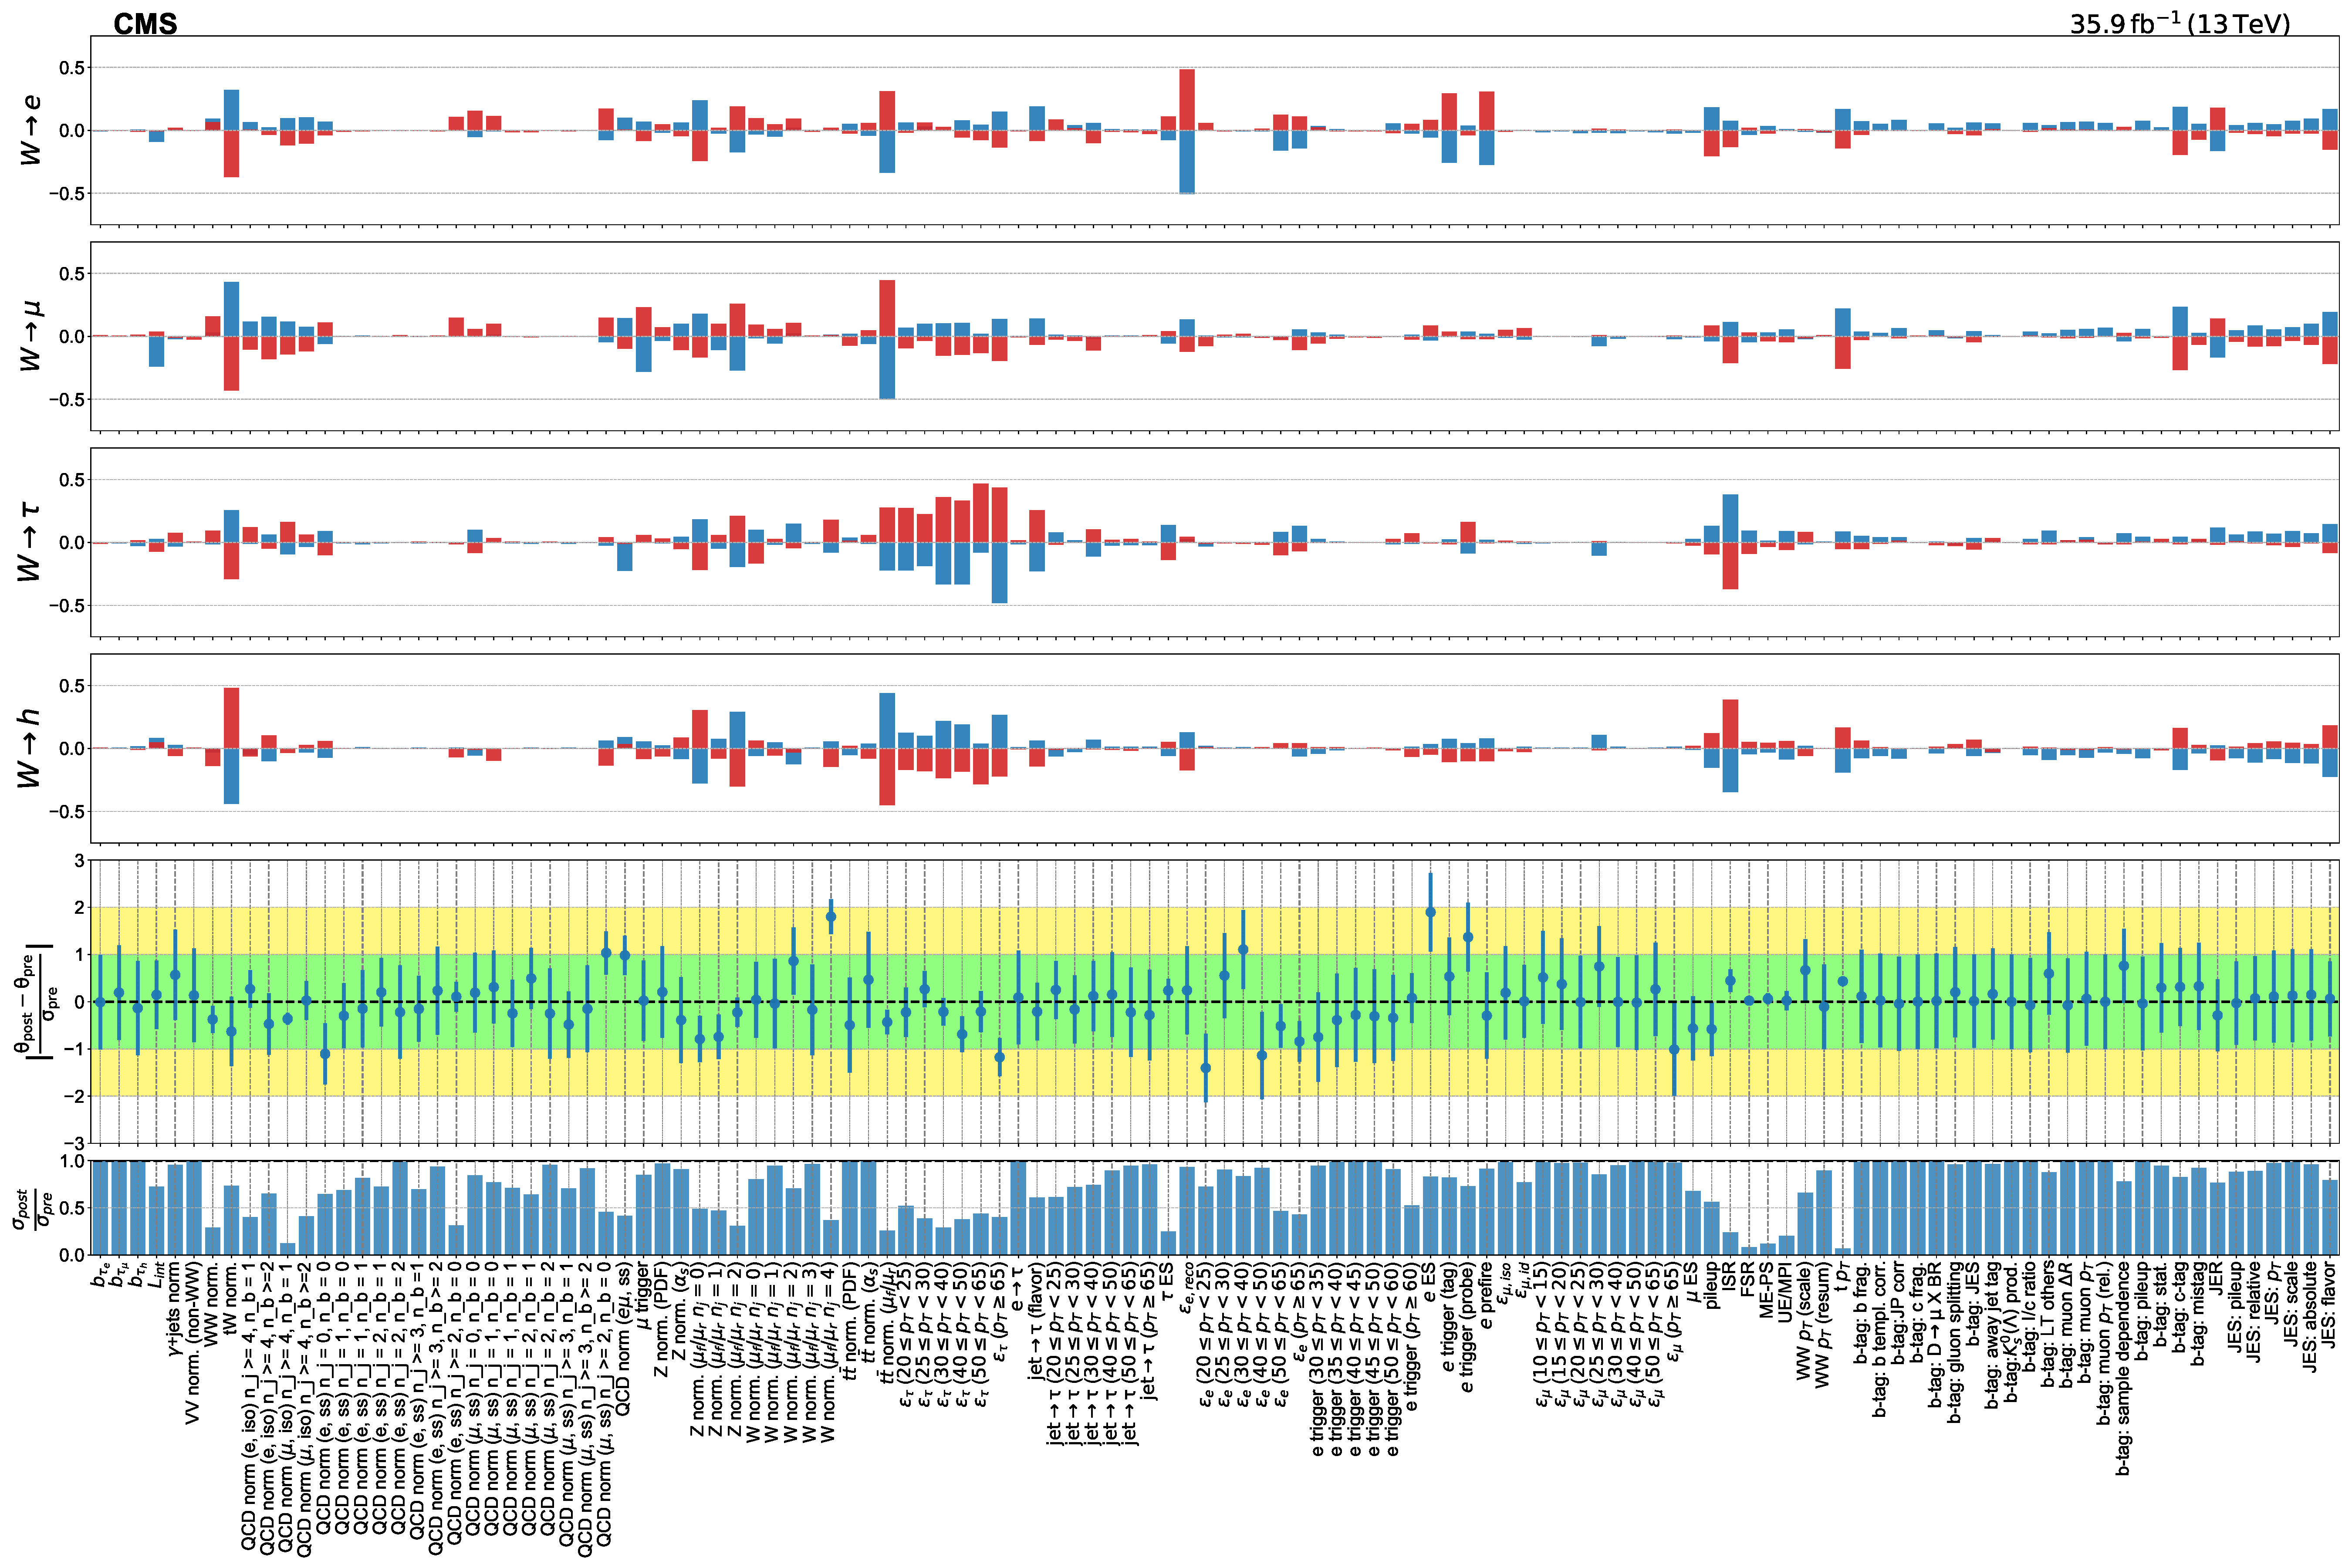
\includegraphics[width=\textwidth]{chapters/Analysis/sectionSystematics/figures/pulls_impacts_final.pdf}
    \caption{Pulls and constrain of all non-MC statistic nuisance
        parameters after minimizing the likelihood.}
    \label{fig:analysis:systematics:pulls_all}
\end{sidewaysfigure}

\begin{figure}[ht]
    \centering
    \includegraphics[width=0.99\textwidth]{chapters/Analysis/sectionSystematics/figures/correlation_matrix_full.pdf}
    \caption{Correlation matrix for branching fractions and nuisance
        parameters.  This does not include the nuisance parameters
        associated with bin-by-bin MC statistical uncertainty.}
    \label{fig:analysis:systematics:corr_matrix}
\end{figure}

% \begin{figure}[ht]
%     \centering
%     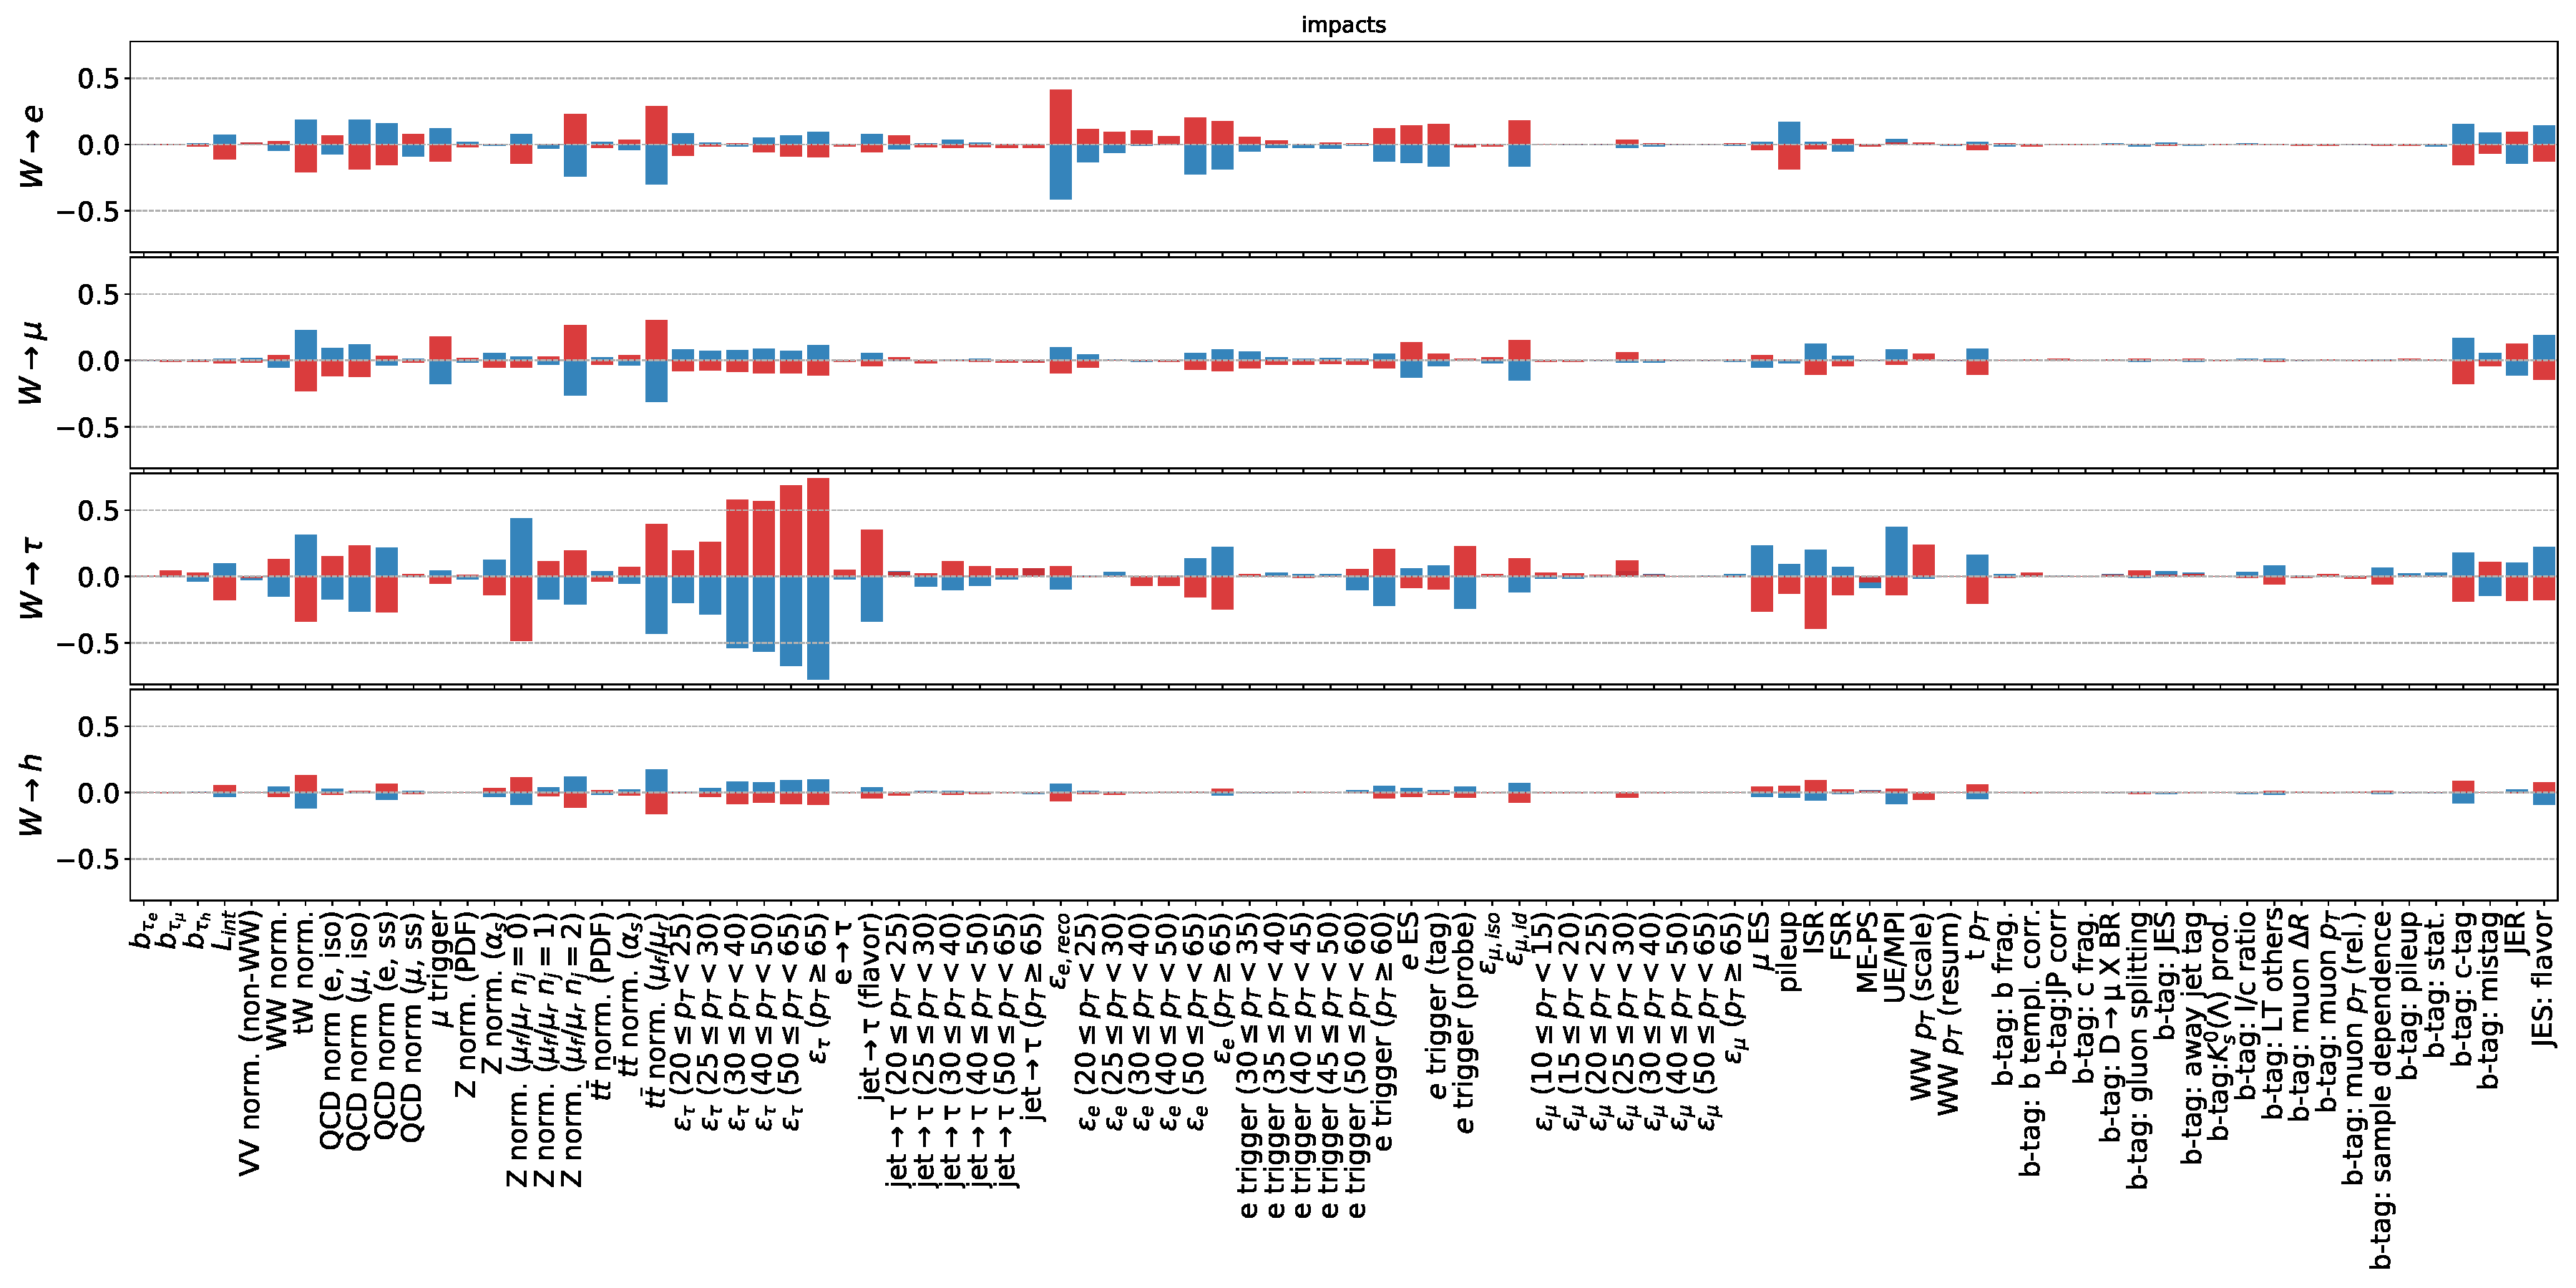
\includegraphics[width=1.2\textwidth, angle=-90]{chapters/Analysis/sectionSystematics/figures/unblinded_impacts.pdf}
%     \caption{impacts}
%     \label{fig:impacts_all}
% \end{figure}

\FloatBarrier



\subsection{Counting Analysis}

For the counting analysis, the systematics are assessed individually by varying up and down the sources of systematic uncertainties. The same branching fraction extraction is repeated with the variated systematic parameter. The change in the branching fractions with respect to the nominal value is treated as the systematic uncertainty resulting from a given source of systematics.

Recall that channels are divided into four groups based on the trigger types and \PQb tag multiplicities, (\gmb, \gmbb, \geb, \gebb), each of which produces one \BWl measurement. Table~\ref{tab:syst_alt} shows the uncertainties of \BWl in these four groups due to each individual source of systematics. The combine of the four groups assumes
\begin{enumerate}
    \item one single source of systematics is fully correlated among the four groups.
    \item different sources of systematics are mutually independent.
\end{enumerate}

\noindent Therefore, the chi-squared in the combine can be written as
\begin{equation}
    \chi^2 (\beta) = (\beta_0 - \textbf{A} \beta )^T \textbf{V}^{-1} (\beta_0 - \textbf{A} \beta )
\end{equation}

\noindent where $\beta = [\bwe, \bwm, \bwt]^T $ is the combined branching fraction, and
$\beta_0$ is the nominal value of the four measurements in the \gmb, \gmbb, \geb, \gebb group, defined as
% 
\begin{equation}
    \beta_0 = \bigg [
    \bwe^{\gmb},  \bwm^{\gmb},  \bwt^{\gmb}, \quad 
    \bwe^{\gmbb}, \bwm^{\gmbb}, \bwt^{\gmbb}, \quad 
    \bwe^{\geb},  \bwm^{\geb},  \bwt^{\geb}, \quad
    \bwe^{\gebb}, \bwm^{\gebb}, \bwt^{\gebb}
    \bigg ]^T,
\end{equation}

\noindent and $\textbf{A}=[I_{3\times3}, I_{3\times3}, I_{3\times3}, I_{3\times3}]^T$ is a $12 \times 3$  matrix consist of four $3\times 3$ identity matrices. $\textbf{V}$ is the variance matrix for the 12 elements in $\beta_0$, which combines the various sources of statistical and the systematic uncertainties.

\begin{equation}
    \textbf{V} =
    \sum_{n \in \text{data,MC}} \big( \Delta_{n}\beta_0 \big) \otimes   \big( \Delta_{n}\beta_0 \big) +
    \sum_{\theta \in \text{syst}} \big( \Delta_{\theta}\beta_0 \big) \otimes  \big( \Delta_{\theta}\beta_0 \big).
\end{equation}

\noindent where $\Delta_{\theta}\beta_0$ is the variation of \BWl with respective to one sigma of systematic parameter $\theta$, and the absolute value of $\Delta_{\theta}\beta_0$ are the shown as rows in Table~\ref{tab:syst_alt}. The statistical and systematic part of the $\textbf{V}$ matrix is shown in Figure~\ref{fig:corBetaBar}. The combined \bwl can be analytically calculated:
\begin{equation}
    \beta =   (\textbf{A}^T \textbf{V}^{-1} \textbf{A})^{-1}(\textbf{A}^T \textbf{V}^{-1}) \beta_0 , \quad
    \text{with } \textbf{Var}\big[\beta\big]  =   (\textbf{A}^T \textbf{V}^{-1} \textbf{A})^{-1}.
\end{equation}

\begin{figure}[ht]
    \centering
    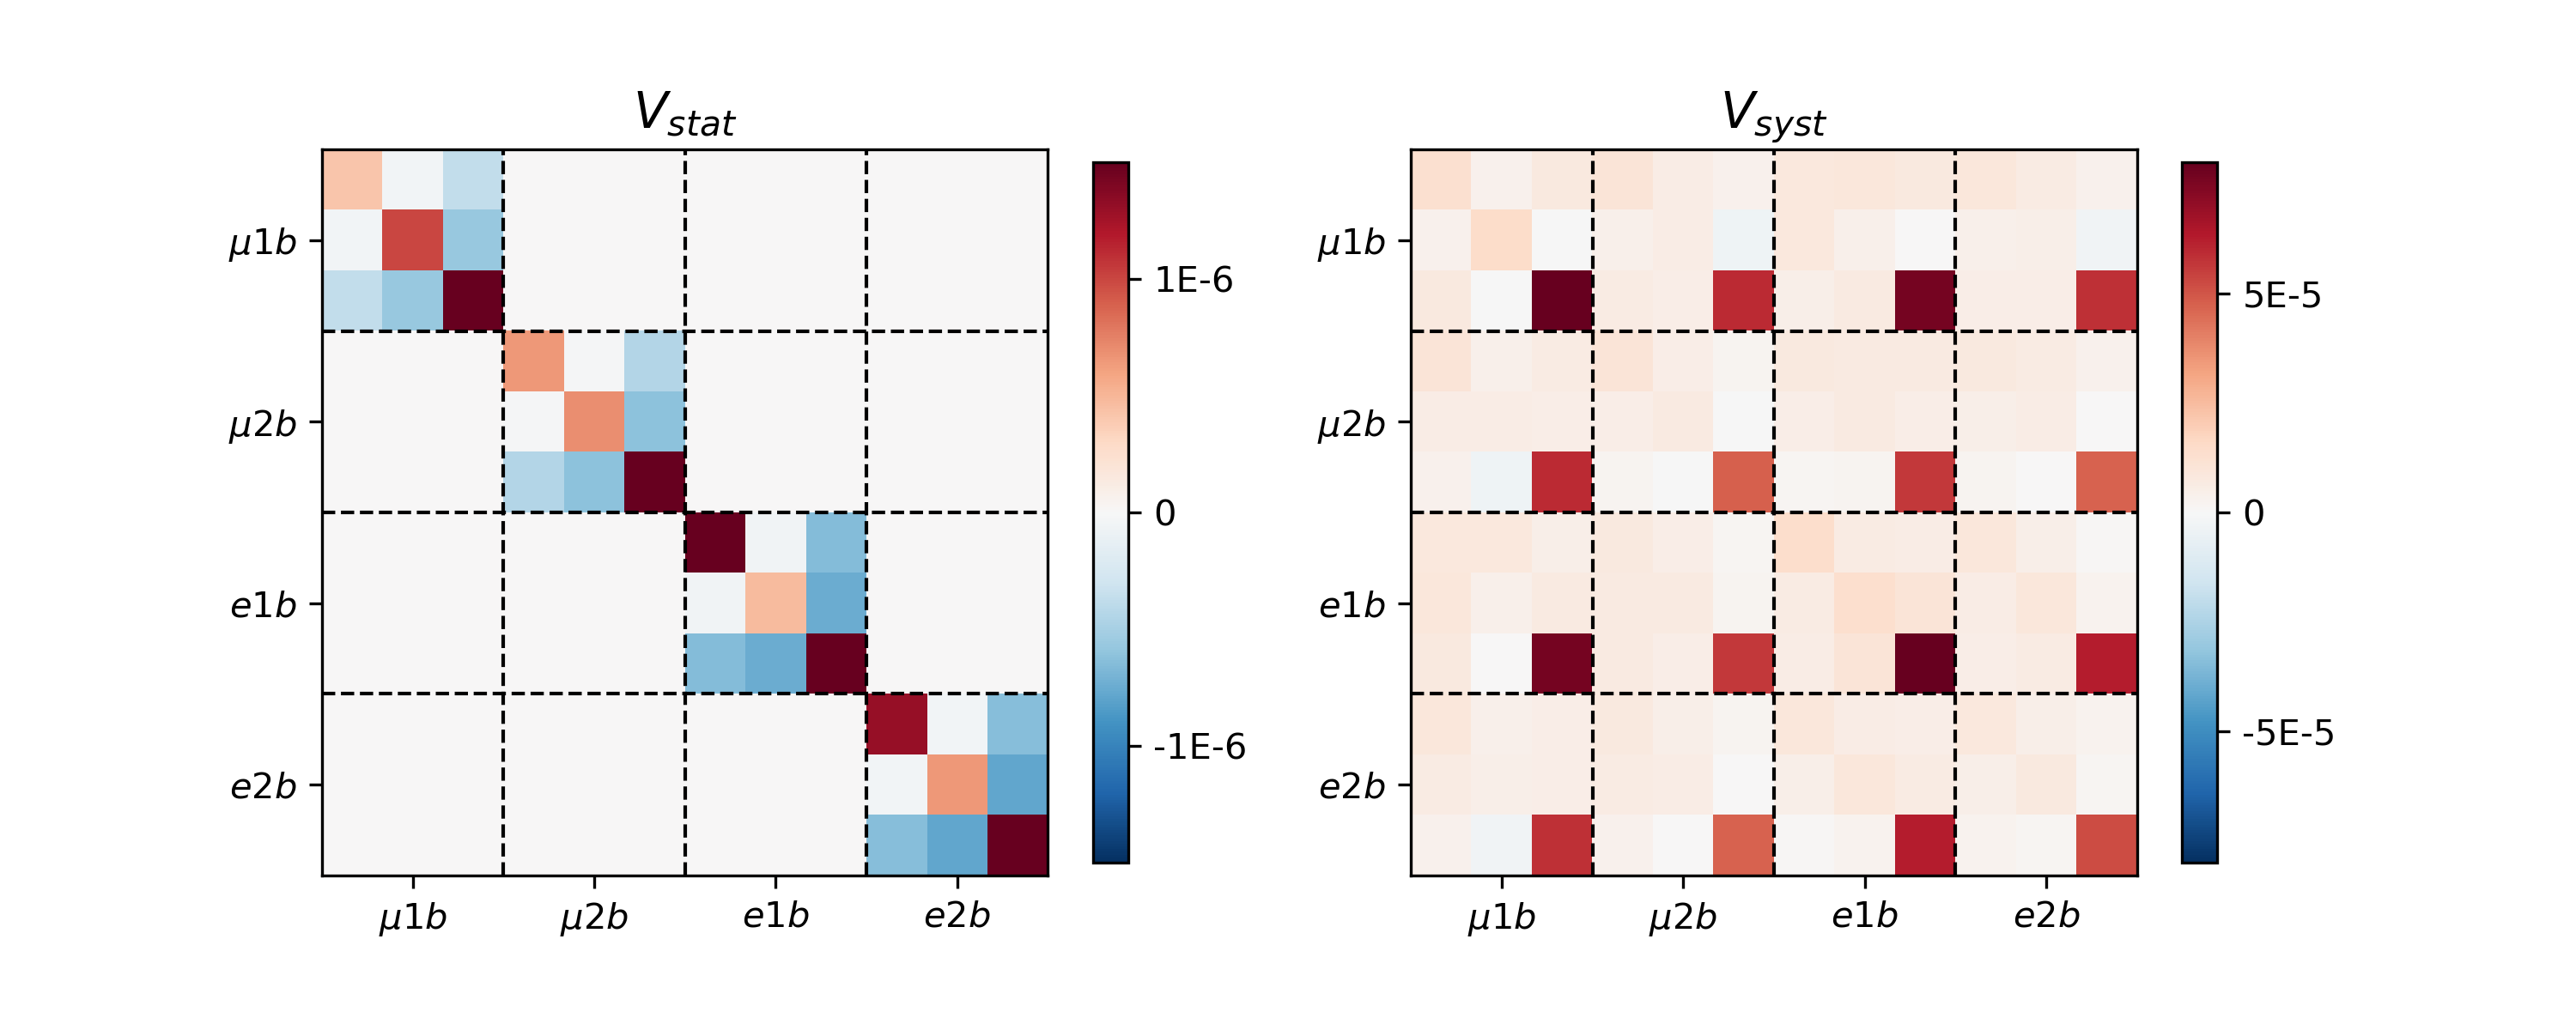
\includegraphics[width=0.99\textwidth]{chapters/Analysis/sectionSystematics/figures/covarMatrix_total.png}
    \caption{ The statistical and systematic part of the $\textbf{V}$ matrix. }
    \label{fig:corBetaBar}
\end{figure}

\begin{sidewaysfigure}[ht]
    \centering
    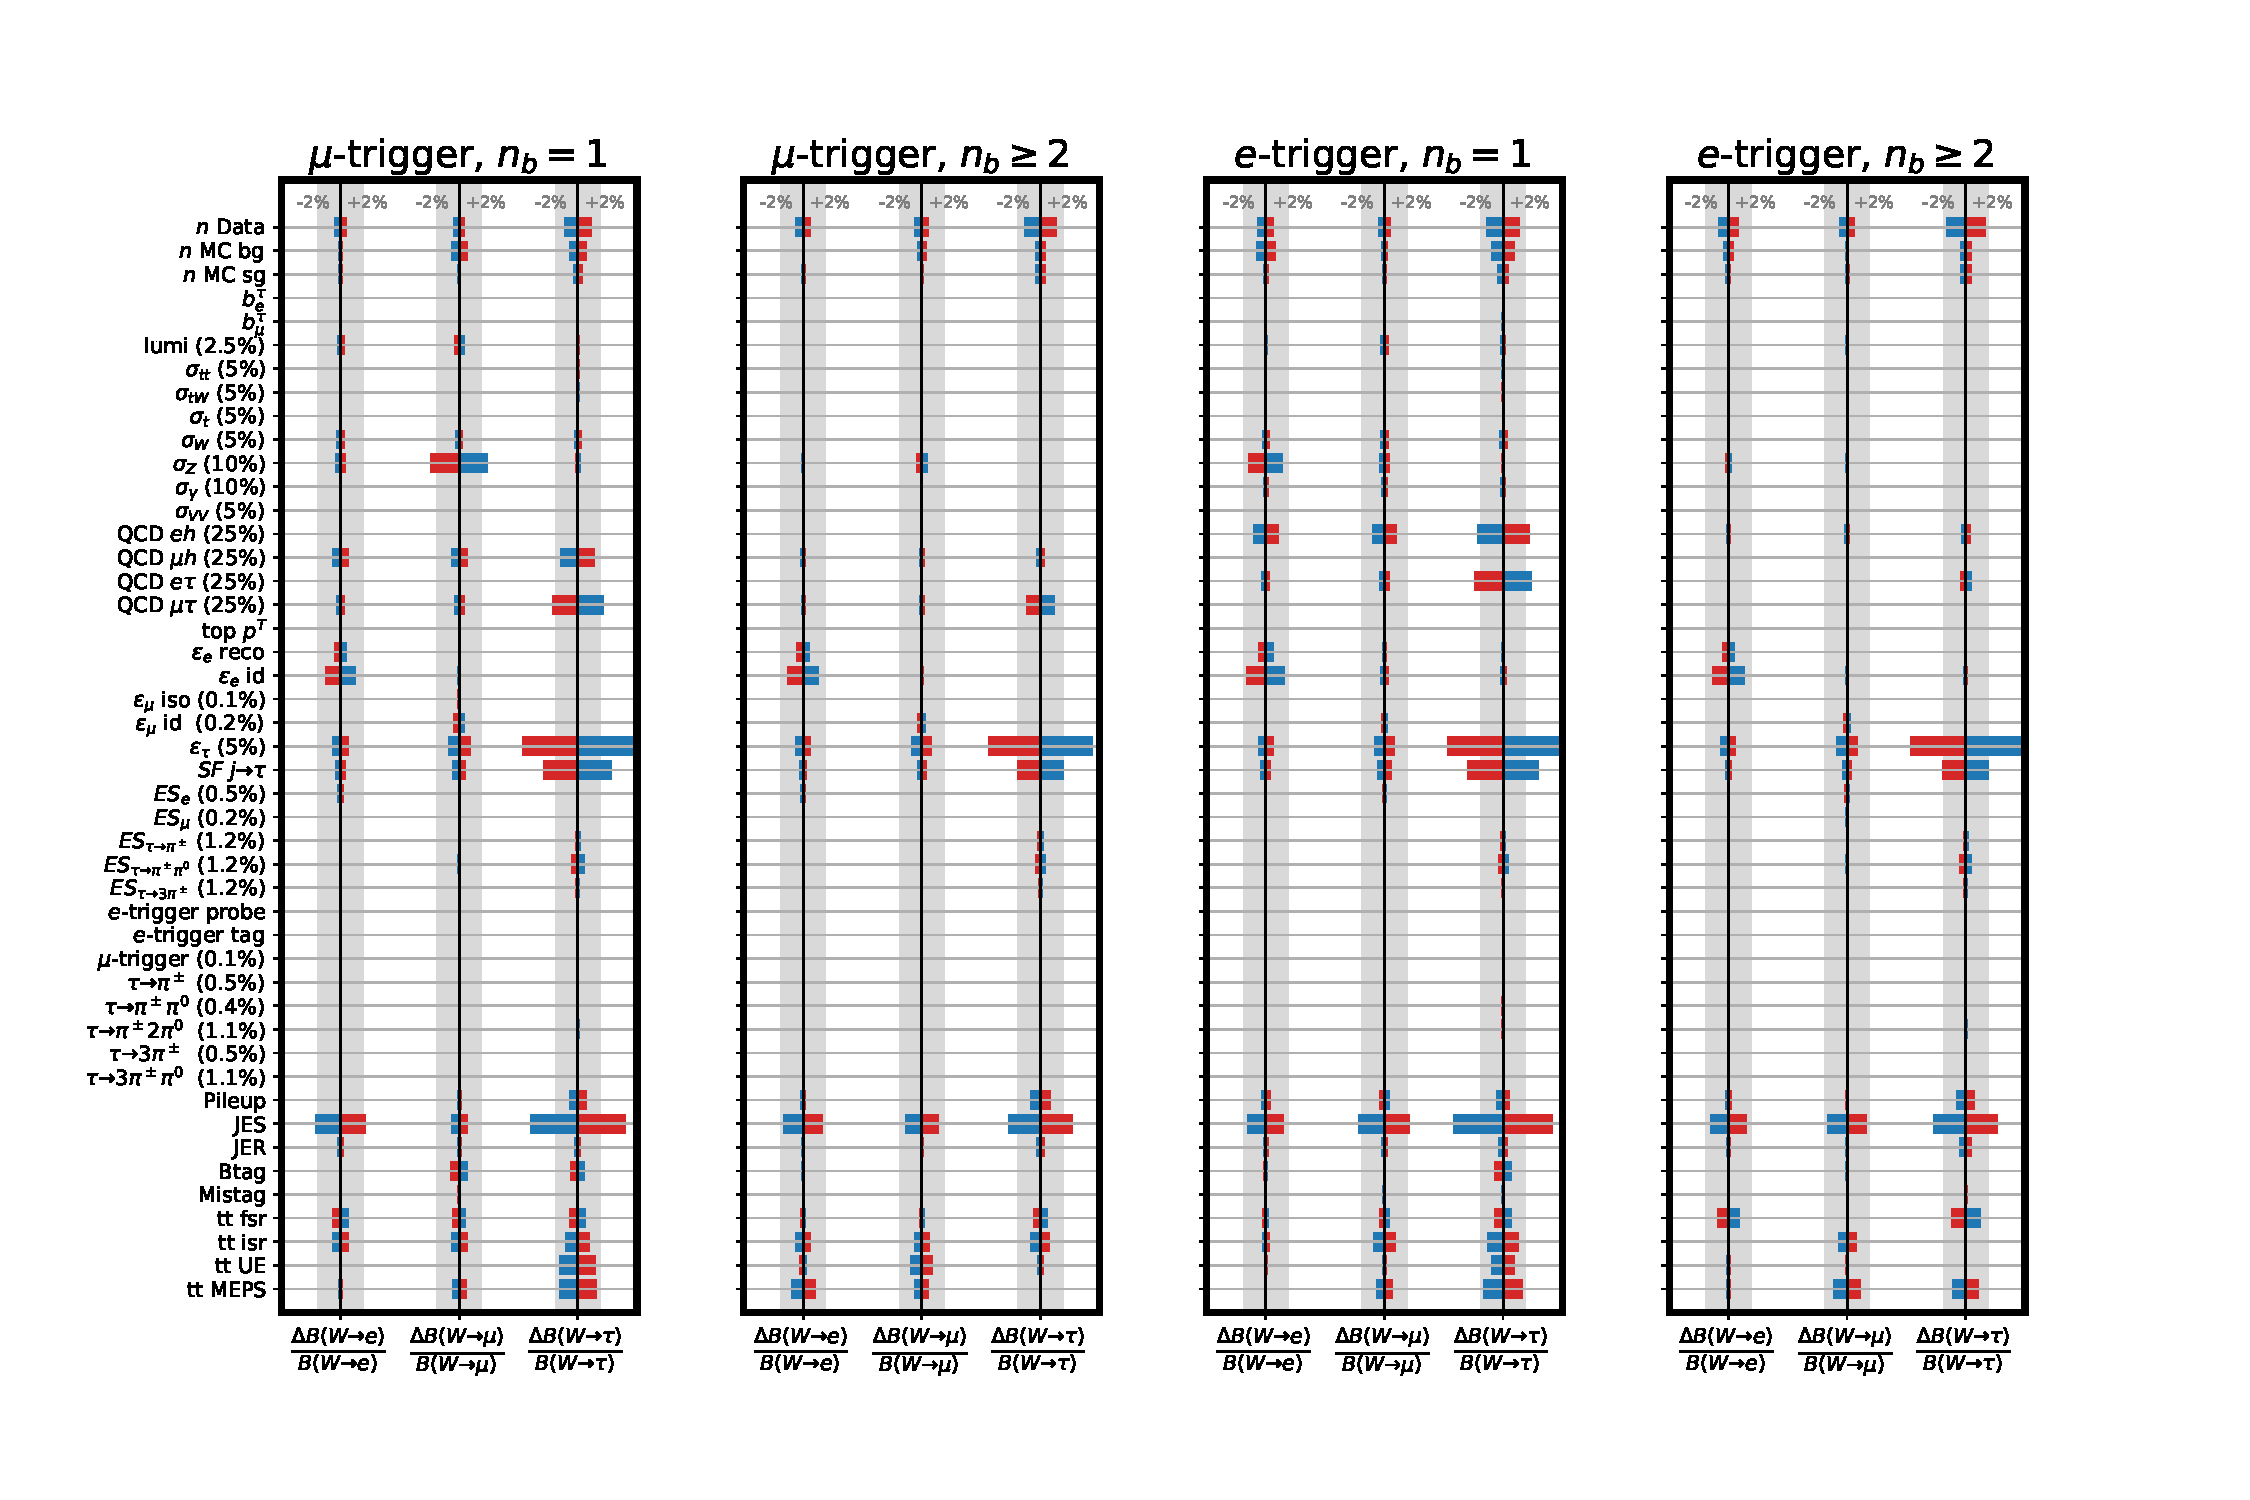
\includegraphics[width=\textwidth]{chapters/Analysis/sectionSystematics/figures/systematics_impact_counting.pdf}
    \caption{Statistical uncertainties and impacts of systematic parameters in counting analysis.}
    \label{fig:analysis:systematics:pulls_all}
\end{sidewaysfigure}

\begin{table}[ht]
  \renewcommand{\arraystretch}{1.1}
  \setlength{\tabcolsep}{0.4em}
  \centering
  \caption{ Statistical and systematic uncertainties in counting analysis. }
  \resizebox{\textwidth}{!}{\begin{table}[]

    
  \renewcommand{\arraystretch}{1.1}
  \setlength{\tabcolsep}{0.4em}
  \centering
  \caption{ Statistical and systematic error of four categories. }
  \resizebox{\textwidth}{!}{
      \begin{tabular}{|l|ccc|ccc|ccc|ccc|ccc|}
      \hline
      Error Source & \multicolumn{3}{c|}{$\mu$-1b} & \multicolumn{3}{c|}{$\mu$-2b} & \multicolumn{3}{c|}{$e$-1b} & \multicolumn{3}{c|}{$e$-2b} \\
      \hline
                    & $B_e$ & $B_\mu$ & $B_\tau$ & $B_e$ & $B_\mu$ & $B_\tau$ & $B_e$ & $B_\mu$ & $B_\tau$ & $B_e$ & $B_\mu$ & $B_\tau$ \\
      \hline
      StatErr of Data                            & 0.543 & 0.533 & 1.243 & 0.714 & 0.637 & 1.492 & 0.743 & 0.557 & 1.520 & 0.904 & 0.707 & 1.807 \\ 
      StatErr of bg MC                           & 0.178 & 0.745 & 0.767 & 0.110 & 0.411 & 0.501 & 0.897 & 0.257 & 1.065 & 0.494 & 0.137 & 0.521 \\ 
      StatErr of sg MC                           & 0.168 & 0.151 & 0.415 & 0.189 & 0.165 & 0.428 & 0.217 & 0.176 & 0.503 & 0.233 & 0.192 & 0.520 \\ 
      \hline
      PDG err of $Br^\tau_e$                     & 0.002 & 0.019 & 0.029 & 0.002 & 0.019 & 0.029 & 0.003 & 0.019 & 0.029 & 0.003 & 0.020 & 0.030 \\ 
      PDG err of $Br^\tau_\mu$                   & 0.047 & 0.017 & 0.098 & 0.047 & 0.017 & 0.099 & 0.041 & 0.013 & 0.101 & 0.043 & 0.013 & 0.106 \\ 
      2.5$\%$ err of luminosity                  & 0.330 & 0.461 & 0.120 & 0.093 & 0.064 & 0.049 & 0.135 & 0.390 & 0.204 & 0.002 & 0.101 & 0.092 \\ 
      5$\%$ err of tt XS                         & 0.002 & 0.000 & 0.151 & 0.009 & 0.015 & 0.032 & 0.021 & 0.011 & 0.148 & 0.011 & 0.002 & 0.003 \\ 
      5$\%$ err of tW XS                         & 0.002 & 0.001 & 0.157 & 0.010 & 0.015 & 0.033 & 0.022 & 0.012 & 0.155 & 0.011 & 0.002 & 0.004 \\ 
      5$\%$ err of t XS                          & 0.062 & 0.062 & 0.033 & 0.053 & 0.052 & 0.058 & 0.063 & 0.060 & 0.032 & 0.052 & 0.054 & 0.040 \\ 
      5$\%$ err of W+Jets XS                     & 0.343 & 0.354 & 0.325 & 0.068 & 0.068 & 0.066 & 0.349 & 0.347 & 0.366 & 0.065 & 0.066 & 0.084 \\ 
      10$\%$ err of Z+Jets XS                    & 0.495 & 2.655 & 0.237 & 0.122 & 0.491 & 0.055 & 1.576 & 0.501 & 0.173 & 0.275 & 0.104 & 0.041 \\ 
      10$\%$ err of $\gamma$+Jets XS             & 0.020 & 0.019 & 0.029 & 0.005 & 0.005 & 0.007 & 0.249 & 0.247 & 0.213 & 0.058 & 0.058 & 0.081 \\ 
      10$\%$ err of VV XS                        & 0.004 & 0.044 & 0.027 & 0.001 & 0.010 & 0.005 & 0.038 & 0.003 & 0.021 & 0.008 & 0.001 & 0.001 \\ 
      25$\%$ err of QCD in $e 4j$                & 0.000 & 0.000 & 0.000 & 0.000 & 0.000 & 0.000 & 1.164 & 1.118 & 2.410 & 0.219 & 0.218 & 0.406 \\ 
      25$\%$ err of QCD in $\mu 4j$              & 0.742 & 0.737 & 1.562 & 0.223 & 0.214 & 0.384 & 0.000 & 0.000 & 0.000 & 0.000 & 0.000 & 0.000 \\ 
      25$\%$ err of QCD in $e\tau$               & 0.000 & 0.000 & 0.000 & 0.000 & 0.000 & 0.000 & 0.372 & 0.498 & 2.651 & 0.069 & 0.092 & 0.503 \\ 
      25$\%$ err of QCD in $\mu\tau$             & 0.345 & 0.465 & 2.360 & 0.185 & 0.250 & 1.285 & 0.000 & 0.000 & 0.000 & 0.000 & 0.000 & 0.000 \\ 
      top pT reweighting                         & 0.000 & 0.000 & 0.032 & 0.002 & 0.003 & 0.007 & 0.004 & 0.002 & 0.031 & 0.002 & 0.000 & 0.001 \\ 
      0.6$\%$ err of $\epsilon_e$ reco           & 0.575 & 0.054 & 0.042 & 0.583 & 0.055 & 0.042 & 0.709 & 0.160 & 0.103 & 0.574 & 0.084 & 0.069 \\ 
      1.4$\%$ err of $\epsilon_e$ id             & 1.386 & 0.129 & 0.101 & 1.410 & 0.133 & 0.101 & 1.766 & 0.335 & 0.275 & 1.456 & 0.163 & 0.197 \\ 
      0.1$\%$ err of $\epsilon_\mu$ reco         & 0.015 & 0.125 & 0.016 & 0.008 & 0.095 & 0.011 & 0.009 & 0.078 & 0.008 & 0.008 & 0.077 & 0.008 \\ 
      0.2$\%$ err of $\epsilon_\mu$ id           & 0.052 & 0.496 & 0.066 & 0.021 & 0.370 & 0.045 & 0.033 & 0.299 & 0.029 & 0.032 & 0.299 & 0.031 \\ 
      5$\%$ err of $\epsilon_\tau$               & 0.745 & 1.004 & 5.091 & 0.694 & 0.937 & 4.823 & 0.723 & 0.967 & 5.146 & 0.700 & 0.937 & 5.111 \\ 
      4.7$\%$ err of $\epsilon_{j\to\tau}$       & 0.460 & 0.620 & 3.145 & 0.307 & 0.414 & 2.129 & 0.458 & 0.613 & 3.260 & 0.290 & 0.388 & 2.115 \\ 
      0.5$\%$ err of $ES_{e}$                    & 0.249 & 0.023 & 0.018 & 0.228 & 0.022 & 0.016 & 0.008 & 0.171 & 0.061 & 0.010 & 0.247 & 0.017 \\ 
      0.2$\%$ err of $ES_{\mu}$                  & 0.095 & 0.092 & 0.033 & 0.093 & 0.092 & 0.035 & 0.013 & 0.116 & 0.011 & 0.012 & 0.114 & 0.012 \\ 
      1.2$\%$ err of $ES_{\tau\to\pi^\pm}$       & 0.034 & 0.046 & 0.232 & 0.035 & 0.047 & 0.244 & 0.034 & 0.046 & 0.245 & 0.030 & 0.040 & 0.216 \\ 
      1.2$\%$ err of $ES_{\tau\to\pi^\pm\pi^0}$  & 0.086 & 0.116 & 0.587 & 0.069 & 0.093 & 0.477 & 0.066 & 0.088 & 0.469 & 0.075 & 0.100 & 0.548 \\ 
      1.2$\%$ err of $ES_{\tau\to3\pi^\pm}$      & 0.026 & 0.035 & 0.175 & 0.026 & 0.034 & 0.177 & 0.024 & 0.032 & 0.172 & 0.024 & 0.032 & 0.176 \\ 
      Single-e Trigger (probe syst)              & 0.218 & 0.020 & 0.016 & 0.222 & 0.021 & 0.016 & 0.029 & 0.032 & 0.004 & 0.036 & 0.004 & 0.009 \\ 
      Single-e Trigger (tag syst)                & 0.495 & 0.046 & 0.036 & 0.503 & 0.047 & 0.036 & 0.063 & 0.088 & 0.080 & 0.037 & 0.013 & 0.038 \\ 
      0.5$\%$ err of $Br_{\tau\to\pi^\pm}$       & 0.008 & 0.011 & 0.047 & 0.009 & 0.012 & 0.050 & 0.008 & 0.011 & 0.047 & 0.009 & 0.012 & 0.055 \\ 
      0.4$\%$ err of $Br_{\tau\to\pi^\pm\pi^0}$  & 0.018 & 0.024 & 0.102 & 0.019 & 0.025 & 0.108 & 0.019 & 0.025 & 0.110 & 0.020 & 0.025 & 0.117 \\ 
      1.1$\%$ err of $Br_{\tau\to\pi^\pm2\pi^0}$ & 0.022 & 0.029 & 0.124 & 0.022 & 0.029 & 0.120 & 0.022 & 0.028 & 0.123 & 0.024 & 0.031 & 0.143 \\ 
      0.5$\%$ err of $Br_{\tau\to3\pi^\pm}$      & 0.015 & 0.021 & 0.094 & 0.017 & 0.022 & 0.102 & 0.016 & 0.021 & 0.100 & 0.017 & 0.022 & 0.106 \\ 
      1.1$\%$ err of $Br_{\tau\to3\pi^\pm\pi^0}$ & 0.009 & 0.011 & 0.043 & 0.010 & 0.012 & 0.046 & 0.009 & 0.011 & 0.043 & 0.010 & 0.012 & 0.046 \\ 
      Pileup                                     & 0.041 & 0.183 & 0.777 & 0.231 & 0.026 & 0.891 & 0.428 & 0.474 & 0.592 & 0.248 & 0.137 & 0.835 \\ 
      JES                                        & 2.300 & 0.750 & 4.421 & 1.823 & 1.543 & 2.968 & 1.681 & 2.370 & 4.577 & 1.681 & 1.773 & 2.993 \\ 
      JER                                        & 0.238 & 0.180 & 0.265 & 0.143 & 0.146 & 0.356 & 0.259 & 0.249 & 0.406 & 0.148 & 0.138 & 0.538 \\ 
      Btag                                       & 0.098 & 0.772 & 0.643 & 0.111 & 0.023 & 0.114 & 0.181 & 0.091 & 0.762 & 0.024 & 0.109 & 0.088 \\ 
      Mistag                                     & 0.100 & 0.141 & 0.035 & 0.100 & 0.056 & 0.090 & 0.077 & 0.142 & 0.124 & 0.030 & 0.096 & 0.135 \\ 
      tt fsr                                     & 0.760 & 0.583 & 0.743 & 0.236 & 0.253 & 0.643 & 0.289 & 0.473 & 0.756 & 1.029 & 0.065 & 1.337 \\ 
      tt isr                                     & 0.724 & 0.747 & 1.105 & 0.720 & 0.723 & 0.876 & 0.317 & 1.060 & 1.414 & 0.043 & 0.830 & 0.062 \\ 
      tt UE                                      & 0.021 & 0.037 & 1.665 & 0.306 & 1.017 & 0.266 & 0.122 & 0.177 & 1.060 & 0.172 & 0.133 & 0.053 \\ 
      tt MEPS                                    & 0.198 & 0.653 & 1.699 & 1.117 & 0.645 & 0.129 & 0.033 & 0.743 & 1.812 & 0.163 & 1.279 & 1.196 \\ 
      \hline
      Total                                      & 3.378 & 3.646 & 8.655 & 3.047 & 2.579 & 6.609 & 3.643 & 3.459 & 9.135 & 2.884 & 2.728 & 6.967 \\ 
      \hline
      \end{tabular}
  }
 
  \label{tab:syst_alt}
\end{table}
}
  \label{tab:syst_alt}
\end{table}







\FloatBarrier



% \subsubsection{Method and Result of Analytic Combining}

% The counting analysis extracts leptonic branching fractions
% $\{\bwe, \bwm, \bwt\}$ simultaneously from yields of mutually exclusive channels, 
% grouped in four trigger-bjet categories, $\mu-1b$,  $\mu-2b$,  $e-1b$ and $e-2b$.
% Its parameter extraction outputs totally 4 sets of $\{\bwe, \bwm, \bwt\}$,
% one set in each category. We denote the output 4 sets of $\{\bwe, \bwm, \bwt\}$
% as a vector $\beta$.

% \begin{equation}
%     \beta = \bigg [
%     \bwe^{\gmb}, \bwm^{\gmb}, \bwt^{\gmb}, \quad 
%     \bwe^{\gmbb}, \bwm^{\gmbb}, \bwt^{\gmbb}, \quad 
%     \bwe^{\geb}, \bwm^{\geb}, \bwt^{\geb}, \quad
%     \bwe^{\gebb}, \bwm^{\gebb}, \bwt^{\gebb}
%     \bigg ]
% \end{equation}

% $\beta$ variates with respect to the statistical fluctuation 
% of event yields, as well as the variation of systematic parameters,
% leading to its statistical and systematic uncertainties.


% The statistical variance of $\beta$ is calculated by propagating 
% the statistical uncertainty of yield in each channel, 
% then summing them in quadrature. As is given in Eqn \ref{eqn:statVar}.
% The summation in quadrature is based on the fact that the statistical 
% fluctuation in each channel is fully independent.

% \begin{equation}
%     \textbf{V}_{stat} = \sum_{i \in ch} 
%     \bigg( \frac{\partial \beta}{\partial n_i} \delta_{n_i} \bigg) \otimes 
%     \bigg( \frac{\partial \beta}{\partial n_i} \delta_{n_i} \bigg)
%     \label{eqn:statVar}
% \end{equation}

% The systematic uncertainty due to a given systematic parameter is
% evaluated by variating this systematic parameter by its 
% own uncertainty and then taking the changes of outcoming $\beta$. 
% The total systematic variance is obtained by summing all systematic 
% uncertainties in quadrature. As is given in Eqn \ref{eqn:systVar}.
% This summation of quadrature is based on the assumption made in counting analysis 
% that all systematic parameters in consideration are independent from each other.


% \begin{equation}
%     \textbf{V}_{syst} = \sum_{\theta \in syst}
%     \big( \Delta_{\theta}\beta \big) \otimes 
%     \big( \Delta_{\theta}\beta \big)
%     \label{eqn:systVar}
% \end{equation}

% The outer product of variations is based on the fact that all elements of
% $\beta$ is fully correlated when tuning up and down a systematic parameters.
% Table \ref{tbl:errors} shows the squared root of diagonal elements of 
% $\textbf{V}_{stat}$ and $\textbf{V}_{syst}$. The full matrix of $\textbf{V}_{stat}$ 
% and $\textbf{V}_{syst}$ are shown in Fig \ref{fig:varStatSyst}.
% The total variance of $\beta$ is summation of statistics and systematics variance.
% The variance matrix not only represents the sensitivity of the measurement 
% to each systematics, but also characterizes the correction among 
% $\{\bwe, \bwm, \bwt\}$ within each category and across all four categories. 

% \begin{equation}
%     \textbf{V} = \textbf{V}_{stat} + \textbf{V}_{syst}
% \end{equation}

% To combine the branching fraction in four categories, we construct $\chi^2$ parametrized
% by average branching fractions, $\bar{\beta}_e,\bar{\beta}_\mu, \bar{\beta}_\PGth$ 
% in Eqn \ref{eqn:DefineChisquared}. 

% \begin{equation}
%     \chi^2 (\bar{\beta}_e, \bar{\beta}_\mu, \bar{\beta}_\PGth) = 
%     (\beta - \bar{\beta} )^T \textbf{V}^{-1} (\beta - \bar{\beta} )
%     \label{eqn:DefineChisquared}
% \end{equation}

% where $\bar{\beta}$ is linearly parametrized by $\bar{\beta}_e, \bar{\beta}_\mu, \bar{\beta}_\PGth$ 
% via a $12 \times 3$ matrix A which consists of four $3\times 3$ identity matrices
% distributing parameters linearly to 4 categories.

% \begin{equation}
%     \bar{\beta} = A \bigg [ \bar{\beta}_e, \bar{\beta}_\mu, \bar{\beta}_\PGth \bigg ]
%     =
%     \bigg [
%     \bar{\beta}_e, \bar{\beta}_\mu, \bar{\beta}_\PGth, \quad 
%     \bar{\beta}_e, \bar{\beta}_\mu, \bar{\beta}_\PGth, \quad 
%     \bar{\beta}_e, \bar{\beta}_\mu, \bar{\beta}_\PGth, \quad 
%     \bar{\beta}_e, \bar{\beta}_\mu, \bar{\beta}_\PGth
%     \bigg ]
% \end{equation}

% Thanks to this linearly parametrizing of $\bar{\beta}$, the first and second 
% derivatives of $\chi^2$ can be calculated analytically.

% \begin{align}
%     &\nabla \chi^2   = -2 (A^T V^{-1} \beta - A^T V^{-1} \bar{\beta} )
%     \\
%     &\nabla^2 \chi^2 = 2 A^T V^{-1} A 
% \end{align}

% The central value of average branching fraction comes from minimizing this $\chi ^2$, or
% $\nabla \chi ^2 = 0$
% The variance of average branching fraction comes from Fisher Information, 
% $I = \frac{1}{2} \nabla^2 \chi^2 $ evaluated at 
% point with the least chi-squared $\bar{\beta}^{LS}$.
% In other words, the covariance of average branching fractions,  
% $U [\bar{\beta}^{LS}]$,
% equals to the inverse of
% Fisher Information at $\bar{\beta} = \bar{\beta}^{LS}$.

% \begin{equation}
%     \bar{\beta}^{LS} =   (A^T V^{-1} A)^{-1}(A^T V^{-1})  \cdot \beta
%     \label{eqn:combineMean}
% \end{equation}

% \begin{equation}
%     U \big[\bar{\beta}^{LS} \big]  =   (A^T V^{-1} A)^{-1}
%     \label{eqn:combineCovar}
% \end{equation}

% These analytic formula for LS estimator of linear parameters in 
% Eqn \ref{eqn:combineMean} and \ref{eqn:combineCovar} are derived as Eqn 7.10 and 7.11
% in Glen Cowan's Statistical Data Analysis.
% With this combining method, the values of average branching 
% fractions are shown in Eqn \ref{eqn:averagebf}. The correlation of 
% $\bar{\beta}_e,\bar{\beta}_\mu, \bar{\beta}_\PGth$ is shown in Fig \ref{fig:corBetaBar}. 

% \begin{align}
%     \bar{\beta}_e^{LS}    &= 0.1080 \times \big[1 \pm 0.37\% \text{ (stat)} \pm 2.06\% \text{ (syst)} \big] \\
%     \bar{\beta}_\mu^{LS}  &= 0.1080 \times \big[1 \pm 0.33\% \text{ (stat)} \pm 2.15\% \text{ (syst)} \big] \\
%     \bar{\beta}_\PGth^{LS} &= 0.1080 \times \big[1 \pm 0.81\% \text{ (stat)} \pm 6.35\% \text{ (syst)} \big]
%     \label{eqn:averagebf}
% \end{align}

% \begin{figure}[ht]
%     \centering
%     % \includegraphics[width=7cm]{section5/figures/covarMatrix_beta.png}
%     \caption{ The correlation of $\bar{\beta}_e,\bar{\beta}_\mu, \bar{\beta}_\PGth$ }
%     \label{fig:corBetaBar}
% \end{figure}




